% MIT License
%
% Copyright (c) 2018 José Nascimento <joseaugustodearaujonascimento@gmail.com>
%
% Permission is hereby granted, free of charge, to any person obtaining a copy
% of this software and associated documentation files (the "Software"), to deal
% in the Software without restriction, including without limitation the rights
% to use, copy, modify, merge, publish, distribute, sublicense, and/or sell
% copies of the Software, and to permit persons to whom the Software is
% furnished to do so, subject to the following conditions:
%
% The above copyright notice and this permission notice shall be included in all
% copies or substantial portions of the Software.
%
% THE SOFTWARE IS PROVIDED "AS IS", WITHOUT WARRANTY OF ANY KIND, EXPRESS OR
% IMPLIED, INCLUDING BUT NOT LIMITED TO THE WARRANTIES OF MERCHANTABILITY,
% FITNESS FOR A PARTICULAR PURPOSE AND NONINFRINGEMENT. IN NO EVENT SHALL THE
% AUTHORS OR COPYRIGHT HOLDERS BE LIABLE FOR ANY CLAIM, DAMAGES OR OTHER
% LIABILITY, WHETHER IN AN ACTION OF CONTRACT, TORT OR OTHERWISE, ARISING FROM,
% OUT OF OR IN CONNECTION WITH THE SOFTWARE OR THE USE OR OTHER DEALINGS IN THE
% SOFTWARE.
\documentclass[
  % -- opções da classe memoir --
  12pt,                 % tamanho da fonte
  openright,            % capítulos começam em pág ímpar (insere página vazia caso preciso)
  twoside,              % para impressão em recto e verso. Oposto a oneside
  a4paper,              % tamanho do papel.
  % -- opções da classe abntex2 --
  sumario=abnt-6027-2012,
  chapter=TITLE,        % títulos de capítulos convertidos em letras maiúsculas
  section=TITLE,        % títulos de seções convertidos em letras maiúsculas
  %subsection=TITLE,    % títulos de subseções convertidos em letras maiúsculas
  %subsubsection=TITLE, % títulos de subsubseções convertidos em letras maiúsculas
  % -- opções do pacote babel --
  english,              % idioma adicional para hifenização
  french,               % idioma adicional para hifenização
  spanish,              % idioma adicional para hifenização
  brazil                % o último idioma é o principal do documento
]{abntex2}

% ---
% Pacotes básicos
% ---

\usepackage{lmodern}        % Usa a fonte Latin Modern
\usepackage{times}          % Usa a fonte Times New Roman
\usepackage[T1]{fontenc}    % Selecao de codigos de fonte.
\usepackage[utf8]{inputenx} % Codificacao do documento (conversão automática dos acentos)
\usepackage{indentfirst}    % Indenta o primeiro parágrafo de cada seção.
\usepackage{color}          % Controle das cores
\usepackage{graphicx}       % Inclusão de gráficos
\usepackage{microtype}      % para melhorias de justificação
% ---

% ---
% Pacotes de citações
% ---
\usepackage[brazilian,hyperpageref]{backref}   % Paginas com as citações na bibl
\usepackage[alf]{abntex2cite}  % Citações padrão ABNT

% ---
% CONFIGURAÇÕES DE PACOTES
% ---

% ---
% Configurações do pacote backref
% Usado sem a opção hyperpageref de backref
\renewcommand{\backrefpagesname}{Citado na(s) página(s):~}
% Texto padrão antes do número das páginas
\renewcommand{\backref}{}
% Define os textos da citação
\renewcommand*{\backrefalt}[4]{
  \ifcase #1 %
    Nenhuma citação no texto.%
  \or
    Citado na página #2.%
  \else
    Citado #1 vezes nas páginas #2.%
  \fi}%
% ---

\usepackage{textcase}
\usepackage[useregional]{datetime2}
\usepackage{datetime2-calc}
\usepackage[normalem]{ulem}

\usepackage[hypcap=true,justification=centering,skip=0cm]{caption}
\usepackage[justification=centering,skip=0cm]{subcaption}

% \usepackage{newpxtext}
\captionsetup[table]{skip=0cm}
\captionsetup[figure]{skip=0cm}
\captionsetup[subfigure]{skip=0cm}

\usepackage{hyphenat}
\usepackage{booktabs}
\usepackage{navigator}
\usepackage{listings}

\usepackage{float}
\usepackage{multirow}
% \usepackage[all]{nowidow}

\usepackage{mdframed}

% \floatplacement{figure}{!htb}
\floatplacement{figure}{H}
\floatplacement{table}{H}

\graphicspath{ {./imagens/} }

\usepackage{enumitem}
% \setlist{itemsep=4pt,parsep=4pt,topsep=8pt,partopsep=4pt}
% \setlist{nosep}

% \floatstyle{boxed}
% \restylefloat{figure}

\usepackage[dvipsnames]{xcolor}

\definecolor{tamarillo}{RGB}{163,20,20}
\definecolor{brightturquoise}{rgb}{0.03, 0.91, 0.87}
\definecolor{malachite}{rgb}{0.04, 0.85, 0.32}

% Redefinição de instruções

\providecommand{\tightlist}{%
  \setlength{\itemsep}{0pt}\setlength{\parskip}{0pt}
}

% \renewcommand{\listingscaption}{Fig.}
% \renewcommand\theFancyVerbLine{\rm{\arabic{FancyVerbLine}}}

% -----
% Declarações de cabecalhos
% -----
% Cabecalho padrao
\makepagestyle{abntbookheadings}
\makeevenhead{abntbookheadings}{}{}{\ABNTEXfontereduzida\thepage}
\makeoddhead{abntbookheadings}{}{}{\ABNTEXfontereduzida\thepage}
%\makeheadrule{abntbookheadings}{\textwidth}{\normalrulethickness}

% Cabecalho do inicio do capitulo
\makepagestyle{abntbookchapfirst}
\makeoddhead{abntbookchapfirst}{}{}{\ABNTEXfontereduzida\thepage}

% Configura layout para elementos textuais
\renewcommand{\textual}{%
  \pagestyle{abntbookheadings}%
  \aliaspagestyle{chapter}{abntbookchapfirst}% customizing chapter pagestyle
  %\nouppercaseheads%
  \bookmarksetup{startatroot}%
}
% ---

\DTMsavedate{mdate}{2018-06-11}
\date{\DTMusedate{mdate}}

\title{EVA: Desenvolvimento de um Chatbot para Escola Virtual de Governo}
\author{Mauro de Carvalho Gonçalves}
\local{\uppercase{Natal-RN}}
\date{2018}
\orientador{Leonardo Ataide Minora}
\instituicao{%
  Instituto Federal do Rio Grande do Norte -- IFRN
  \par
  Diretoria de Gestão e Tecnologia da Informação -- DIATINF
  \par
  Curso de Tecnologia em Análise e Desenvolvimento de Sistemas -- TADS
}
\tipotrabalho{TCC (Graduação)}
% O preambulo deve conter o tipo do trabalho, o objetivo,
% o nome da instituição e a área de concentração
\preambulo{%
Trabalho de conclusão de curso apresentado ao Curso Superior de Tecnologia em Análise e Desenvolvimento de Sistemas da Diretoria de Gestão e Tecnologia da Informação do Instituto Federal de Educação, Ciência e Tecnologia do Rio Grande do Norte como requisito parcial à obtenção do título de Tecnólogo em Análise e Desenvolvimento de Sistemas.
}

\makeatletter
\hypersetup{
  pdftitle={\@title},
  pdfauthor={\@author},
  pdfsubject={\imprimirpreambulo},
  pdfkeywords={PALAVRAS}{CHAVE}{EM}{PORTUGUES},
  pdfcreator={LaTeX with abnTeX2},
  colorlinks=false,
  linkcolor=blue,
  citecolor=blue,
  urlcolor=blue
}
\makeatother

% ---
% Posiciona figuras e tabelas no topo da página quando adicionadas sozinhas
% em um página em branco. Ver https://github.com/abntex/abntex2/issues/170
\makeatletter
\setlength{\@fptop}{5pt} % Set distance from top of page to first float
\makeatother
% ---

\newcommand{\mfonte}[0]{%
  \fonte{Elaboração própria em \DTMfetchyear{mdate}}}

\newcommand{\mcaption}[1]
{%
  \caption[#1]{%
    #1
  }
}

\newcommand{\alusao}[1]{\citeauthor{#1}~(\citeyear{#1})}

\mdfsetup{
  leftmargin=0cm,
  skipabove=0cm,
  rightmargin=0cm,
  skipbelow=0cm,
  innertopmargin=.1cm,
  innerrightmargin=.1cm,
  innerleftmargin=.1cm,
  innerbottommargin=.1cm,
}

\newlength{\MaxSizeOfLineNumbers}%
% Adjust to maximum number of lines
\settowidth{\MaxSizeOfLineNumbers}{99}%
\addtolength{\MaxSizeOfLineNumbers}{2.5ex}%
\lstset{
  showstringspaces=false,
  numbers=left,
  numbersep=2.5ex,
  xleftmargin=\MaxSizeOfLineNumbers,
  keywordstyle=\color{blue},
  basicstyle=\ttfamily,
  breaklines=true,
  stringstyle=\color{tamarillo},
  literate=
    {á}{{\'a}}1
    {à}{{\`a}}1
    {é}{{\'e}}1
    {ê}{{\^e}}1
    {ã}{{\~a}}1
    {ó}{{\'o}}1
    {ç}{{\c{c}}}1%
}
\renewcommand\sout[1]{}
\usepackage[export]{adjustbox}

\let\oldincludegraphics\includegraphics
\renewcommand{\includegraphics}[2][]{%
  \begin{mdframed}%
%   \begin{center}%
    \centering%
    \oldincludegraphics[max width=.7\linewidth,#1]{#2}%
%   \end{center}%
  \end{mdframed}%
}

\setlength{\ABNTEXsignwidth}{10cm}

% ---
% Espaçamentos entre linhas e parágrafos
% ---

% O tamanho do parágrafo é dado por:
\setlength{\parindent}{1.3cm}

% Controle do espaçamento entre um parágrafo e outro:
\setlength{\parskip}{0.2cm}  % tente também \onelineskip

% \renewcommand{\ABNTEXchapterfont}{\bfseries}
% \newcommand{\ABNTEXpartfont}{\ABNTEXchapterfont}
%
% Fontes das entradas do sumario
%
% \renewcommand{\cftpartfont}{\bfseries\larger}

\renewcommand*{\cftchapterleader}{\hfill}
\renewcommand*{\cftsectionleader}{\hfill}
\renewcommand*{\cftsubsectionleader}{\hfill}
\renewcommand*{\cftsubsubsectionleader}{\hfill}

\setlength{\cftbeforechapterskip}{0em}

\renewcommand{\cftchapterfont}{\bfseries}
\renewcommand{\cftchapterpagefont}{\normalsize\normalfont}

\renewcommand{\cftsectionfont}{\normalfont}
\renewcommand{\cftsectionpagefont}{\normalsize\normalfont}

\renewcommand{\cftsubsectionpagefont}{\normalsize\normalfont}

\renewcommand{\cftsubsubsectionfont}{\normalfont}
\renewcommand{\cftsubsubsectionpagefont}{\normalsize\normalfont}

\makeatletter
\let\oldcontentsline\contentsline
\def\contentsline#1#2{%
  \expandafter\ifx\csname l@#1\endcsname\l@section
  \expandafter\@firstoftwo
  \else
  \expandafter\@secondoftwo
  \fi
  {%
    \oldcontentsline{#1}{\MakeTextUppercase{#2}}%
  }{%
  \oldcontentsline{#1}{#2}%
}%
}
\makeatother

% \renewcommand{\cftsubsectionfont}{\bfseries}
% \renewcommand{\cftsubsectionpagefont}{\normalsize\cftsubsectionfont}

% \renewcommand{\cftsubsubsectionfont}{\normalsize}
% \renewcommand{\cftsubsubsectionpagefont}{\cftsubsubsectionfont}

% \renewcommand{\cftparagraphfont}{\footnotesize}
% \renewcommand{\cftparagraphpagefont}{\cftparagraphfont}

%
% Fontes das seções/capítulos
%
\renewcommand{\ABNTEXpartfontsize}{\normalsize}

\renewcommand{\ABNTEXchapterfont}{\bfseries}
\renewcommand{\ABNTEXchapterfontsize}{\normalsize}

\renewcommand{\ABNTEXsectionfont}{\normalsize}
\renewcommand{\ABNTEXsectionfontsize}{\normalsize}

\renewcommand{\ABNTEXsubsectionfont}{\bfseries}
\renewcommand{\ABNTEXsubsectionfontsize}{\normalsize}

\renewcommand{\ABNTEXsubsubsectionfont}{\normalsize}
\renewcommand{\ABNTEXsubsubsectionfontsize}{\normalsize}

\renewcommand{\ABNTEXsubsubsubsectionfontsize}{\normalsize}

% \newcommand{\ABNTEXsectionfont}{\ABNTEXchapterfont}
% \newcommand{\ABNTEXsubsectionfont}{\ABNTEXsectionfont}
% \newcommand{\ABNTEXsubsubsectionfont}{\ABNTEXsubsectionfont}
% \newcommand{\ABNTEXsubsubsubsectionfont}{\ABNTEXsubsectionfont}

% ---
% compila o indice
% ---
\makeindex

% \setlength{\parindent}{1pt}
\setlength{\parskip}{0pt}

\setlength{\beforechapskip}{1.0\onelineskip}
\setlength{\afterchapskip}{1.0\onelineskip}

\setlength{\beforesecskip}{1.0\onelineskip}
\setlength{\aftersecskip}{1.0\onelineskip}

\setlength{\beforesubsecskip}{1.0\onelineskip}
\setlength{\aftersubsecskip}{1.0\onelineskip}

\setlength{\textfloatsep}{1.0\onelineskip}
\setlength{\floatsep}{1.0\onelineskip}
\setlength{\intextsep}{1.0\onelineskip}

% \setlength{\abovecaptionskip}{0pt}
% \setlength{\belowcaptionskip}{0pt}

% Inicio do documento
\begin{document}
  \selectlanguage{brazil}
  \frenchspacing

  \frontmatter

  % Capa
\begin{titlepage}
	\begin{center}
		
		  
		\begin{minipage}{11.15cm}
			\begin{center}
				\begin{espacosimples}
					{\small \ \\
                       \textsc{Instituto Federal do Rio Grande do Norte}
                       \\
							  \textsc{Campus Natal - Central}					\\
							  \textsc{Diretoria de Gestão e Tecnologia da Informação}	   
							  \\
							  \textsc{Tecnologia em Análise e Desenvolvimento de Sistemas}}   	
                       \\
				\end{espacosimples}
			\end{center}
		\end{minipage}

			
		\vspace{6cm}
						
		% T�tulo do trabalho
		{\setlength{\baselineskip}%
		{1.3\baselineskip}
		{\LARGE \textbf{EVA: Desenvolvimento de um Chatbot para Escola Virtual do Governo}}\par}
			
		\vspace{3cm}
			
		% Nome do aluno (autor)
		{\large \textbf{Mauro de Carvalho Gonçalves}}
						
		\vspace{6cm}
		
		% Local da institui��o onde o trabalho deve ser apresentado e ano de entrega do mesmo
		Natal-RN\\Junho de 2018
	\end{center}
\end{titlepage}
  % MIT License
%
% Copyright (c) 2018 José Nascimento <joseaugustodearaujonascimento@gmail.com>
%
% Permission is hereby granted, free of charge, to any person obtaining a copy
% of this software and associated documentation files (the "Software"), to deal
% in the Software without restriction, including without limitation the rights
% to use, copy, modify, merge, publish, distribute, sublicense, and/or sell
% copies of the Software, and to permit persons to whom the Software is
% furnished to do so, subject to the following conditions:
%
% The above copyright notice and this permission notice shall be included in all
% copies or substantial portions of the Software.
%
% THE SOFTWARE IS PROVIDED "AS IS", WITHOUT WARRANTY OF ANY KIND, EXPRESS OR
% IMPLIED, INCLUDING BUT NOT LIMITED TO THE WARRANTIES OF MERCHANTABILITY,
% FITNESS FOR A PARTICULAR PURPOSE AND NONINFRINGEMENT. IN NO EVENT SHALL THE
% AUTHORS OR COPYRIGHT HOLDERS BE LIABLE FOR ANY CLAIM, DAMAGES OR OTHER
% LIABILITY, WHETHER IN AN ACTION OF CONTRACT, TORT OR OTHERWISE, ARISING FROM,
% OUT OF OR IN CONNECTION WITH THE SOFTWARE OR THE USE OR OTHER DEALINGS IN THE
% SOFTWARE.

\begin{folhaderosto}
%\imprimirfolhaderosto{}

  \begin{center}
    \MakeUppercase{\imprimirautor}

    \vspace*{\fill}\vspace*{\fill}
    \begin{center}
      \MakeUppercase{\imprimirtitulo}
    \end{center}
    \vspace*{\fill}\vspace*{\fill}
  \end{center}

  %\vspace*{\fill}

  \hspace*{\fill}
  \begin{minipage}{.5\textwidth}
    \SingleSpace
    \imprimirpreambulo
    \\[\baselineskip]
    Orientador: M.e \imprimirorientador
  \end{minipage}

  \vspace*{\fill}\vspace*{\fill}
  \vspace*{\fill}\vspace*{\fill}
  \vspace*{\fill}\vspace*{\fill}
  \vspace*{\fill}\vspace*{\fill}

  \begin{center}
      \imprimirlocal{}\\
      \imprimirdata
      \par
  \end{center}

\end{folhaderosto}
%--

  % Folha de aprova��o
\begin{folhadeaprovacao}
	\setlength{\ABNTsignthickness}{0.4pt}
	\setlength{\ABNTsignwidth}{10cm}
	
	\noindent 
	Trabalho de Conclusão de Curso de Graduação sob o título
	\textit{EVA: Desenvolvimento de um Chatbot para Escola Virtual de Governo} apresentada por Mauro de Carvalho Gonçalves e aceita pelo Diretoria
	de Gestão e Tecnologia da Informação do Instituto Federal do Rio Grande do
	Norte, sendo aprovada por todos os membros da banca examinadora abaixo especificada:
		
	% Membros da banca examinadora e respectivas filia��es
	\assinatura
	{
		Me. Leonardo Ataide Minora   			                  \\
		{\small Orientador}											          \smallskip\\ 
		{\footnotesize
			DIATINF -- Diretoria Acadêmica de Gestão e Tecnologia da Informação		   \\
		  	IFRN -- Instituto Federal de Educação, Ciência e Tecnologia do Rio Grande do Norte
		}
   }
      
   \assinatura
	{
      Me. José Antônio da Cunha   			                  \\
		{\small Examinador}											          \smallskip\\ 
		{\footnotesize
			DIATINF -- Diretoria Acadêmica de Gestão e Tecnologia da Informação		   \\
		  	IFRN -- Instituto Federal de Educação, Ciência e Tecnologia do Rio Grande do Norte
		}
   }   
   
   \assinatura
	{
      Bruno Pereira Pontes 			                  \\
		{\small Examinador}											          \smallskip\\ 
		{\footnotesize
			DIAC -- Diretoria Acadêmica		\\
		  	IFRN -- Instituto Federal de Educação, Ciência e Tecnologia do Rio Grande do Norte
		}
	}
		
	\vfill
	
	\begin{center}
		Natal-RN, 11/06/2018.
	\end{center}
\end{folhadeaprovacao}

  % MIT License
%
% Copyright (c) 2018 José Nascimento <joseaugustodearaujonascimento@gmail.com>
%
% Permission is hereby granted, free of charge, to any person obtaining a copy
% of this software and associated documentation files (the "Software"), to deal
% in the Software without restriction, including without limitation the rights
% to use, copy, modify, merge, publish, distribute, sublicense, and/or sell
% copies of the Software, and to permit persons to whom the Software is
% furnished to do so, subject to the following conditions:
%
% The above copyright notice and this permission notice shall be included in all
% copies or substantial portions of the Software.
%
% THE SOFTWARE IS PROVIDED "AS IS", WITHOUT WARRANTY OF ANY KIND, EXPRESS OR
% IMPLIED, INCLUDING BUT NOT LIMITED TO THE WARRANTIES OF MERCHANTABILITY,
% FITNESS FOR A PARTICULAR PURPOSE AND NONINFRINGEMENT. IN NO EVENT SHALL THE
% AUTHORS OR COPYRIGHT HOLDERS BE LIABLE FOR ANY CLAIM, DAMAGES OR OTHER
% LIABILITY, WHETHER IN AN ACTION OF CONTRACT, TORT OR OTHERWISE, ARISING FROM,
% OUT OF OR IN CONNECTION WITH THE SOFTWARE OR THE USE OR OTHER DEALINGS IN THE
% SOFTWARE.

\begin{dedicatoria}
\vspace*{\fill}
\begingroup
\leftskip=4cm
\noindent%
Dedico esse trabalho à minha avó, Lauricy Luz, e ao meu pai, Márcio Jeferson, com todo meu amor e gratidão, por tudo que fizeram por mim ao longo de minha vida. Desejo poder ter sido merecedor do esforço dedicado por vocês em todos os aspectos, especialmente quanto à minha formação.%
\par
\endgroup
\end{dedicatoria}
%--

  % Agradecimentos

\chapter*{Agradecimentos}

Agradecimentos dirigidos àqueles que contribuíram de maneira relevante à
elaboração do trabalho, sejam eles pessoas ou mesmo organizações.


  % Ep�grafe (cita��o seguida de indica��o de autoria)

\chapter*{}
\vspace{15cm}
\begin{flushright}
	\textit
	{
		Citação
	}\medskip\\ 
	Autor
\end{flushright}

  % Resumo
\begin{center}
	{\Large{\textbf{EVA: Desenvolvimento de um \textit{Chatbots} para Escola Virtual do Governo}}}
\end{center}

\vspace{1cm}

\begin{flushright}
	Autor: Mauro de Carvalho Gonçalves\\
	Orientador(a): Leonardo Ataide Minora
\end{flushright}

\vspace{1cm}

\begin{center}
	\Large{\textsc{\textbf{Resumo}}}
\end{center}

\noindent A Escola Virtual do Governo (EV.G) é uma iniciativa que consiste em um portal único para oferta de capacitação a distância voltado a servidores públicos e cidadãos de todo o país.
A EV.G oferece cursos a distância de diferentes instituições e com diferentes temáticas ligadas à administração pública e a cidadania, viabilizando o desafio de contribuir para a formação e o desenvolvimento de milhares de servidores públicos bem como dos cidadãos.
Contudo, o EV.G ainda não dispõe de um central de atendimento aos alunos propriamente dita, e em ambientes de oferta massiva de cursos, o atendimento ao usuário pode ser considerado um diferencial competitivo.
Com o avanço tecnológico, soluções inovadoras e de baixo custo estão surgindo a todo momento. No cenário do atendimento on-line, o uso de \textit{chatbots} é uma opção de baixo custo e alto desempenho. 
Neste contexto de atendimento massivo, foi desenvolvido um \textit{chatbot} de conversação textual para a plataforma de mensagens instantâneas chamada Telegram, denominado de EVA (Enap Virtual Assistant). O objetivo geral de EVA é ter a capacidade de conversar via texto com alunos da EV.G no atendimento administrativo de uma secretaria acadêmica.


\noindent\textit{Palavras-chave}: \textit{Chatbot}, Atendimento ao cliente, Atendimento on-line.
  % Resumo em l�ngua estrangeira (em ingl�s Abstract, em espanhol Resumen, em franc�s R�sum�)
\begin{center}
	{\Large{\textbf{EVA: Development of a Chatbot for Escola Virtual do Governo}}}
\end{center}

\vspace{1cm}

\begin{flushright}
	Author: Mauro de Carvalho Gonçalves\\
	Supervisor: Leonardo Ataide Minora
\end{flushright}

\vspace{1cm}

\begin{center}
	\Large{\textsc{\textbf{Abstract}}}
\end{center}

\noindent The Escola Virtual do Governo (EV.G) is an initiative that consists of a single portal to offer distance training aimed at public servants and citizens from all over the country.
EV.G offers distance courses from different institutions and with different themes related to public administration and citizenship, making it possible to contribute to the training and development of thousands of civil servants as well as citizens.
However, the EV.G still does not have a student service center per se, and in environments where there are massive courses, user service can be considered a competitive differential.
With technological advancement, innovative and low-cost solutions are emerging at all times. In the online service scenario, the use of \textit{chatbots} is a low-cost, high-performance option.
In this context of mass service, a textual conversation chatbot was developed for the instant messaging platform called Telegram called the EVA (EV.G Virtual Assistant). The general objective of EVA is to have the ability to converse via text with EV.G students in the administrative service of an academic secretariat.

\noindent\textit{Keywords}: \textit{Chatbot}, Customer Service, Online Customer Service.

  % ---
  % inserir lista de ilustrações
  % ---
  \pdfbookmark[0]{\listfigurename}{lof}
  \listoffigures*
  \cleardoublepage
  % ---

  % ---
  % inserir lista de tabelas
  % ---
  \pdfbookmark[0]{\listtablename}{lot}
  \listoftables*
  \cleardoublepage
  % ---

  % MIT License
%
% Copyright (c) 2018 José Nascimento <joseaugustodearaujonascimento@gmail.com>
%
% Permission is hereby granted, free of charge, to any person obtaining a copy
% of this software and associated documentation files (the "Software"), to deal
% in the Software without restriction, including without limitation the rights
% to use, copy, modify, merge, publish, distribute, sublicense, and/or sell
% copies of the Software, and to permit persons to whom the Software is
% furnished to do so, subject to the following conditions:
%
% The above copyright notice and this permission notice shall be included in all
% copies or substantial portions of the Software.
%
% THE SOFTWARE IS PROVIDED "AS IS", WITHOUT WARRANTY OF ANY KIND, EXPRESS OR
% IMPLIED, INCLUDING BUT NOT LIMITED TO THE WARRANTIES OF MERCHANTABILITY,
% FITNESS FOR A PARTICULAR PURPOSE AND NONINFRINGEMENT. IN NO EVENT SHALL THE
% AUTHORS OR COPYRIGHT HOLDERS BE LIABLE FOR ANY CLAIM, DAMAGES OR OTHER
% LIABILITY, WHETHER IN AN ACTION OF CONTRACT, TORT OR OTHERWISE, ARISING FROM,
% OUT OF OR IN CONNECTION WITH THE SOFTWARE OR THE USE OR OTHER DEALINGS IN THE
% SOFTWARE.

\begin{siglas}
\OnehalfSpacing
  \item[API] \textit{Application Programming Interface}
  \item[ARM] \textit{Advanced} RISC \textit{Machine}
  \item[CPU] \textit{Central Processing Unit}
  \item[DLL] \textit{Dynamic-link Library}
  \item[ECMA] \textit{European Computer Manufacturers Association}
  \item[ENIAC] \textit{Electronic Numerical Integrator and Computer}
  \item[GCC] GNU \textit{Compiler Collection}
  \item[GNU] GNU \textit{is Not Unix}
  \item[IDE] \textit{Integrated Development Environment}
  \item[IFRN] Instituto Federal do Rio Grande do Norte
  \item[RAM] \textit{Random Access Memory}
  \item[RISC] \textit{Reduced Instruction Set Computer}
  \item[TADS] Tecnologia em Análise e Desenvolvimento de Sistemas
\end{siglas}
%--

  % ---
  % inserir o sumario
  % ---
  \pdfbookmark[0]{\contentsname}{toc}
  \tableofcontents*
  \cleardoublepage
  % ---

  % Parte central do trabalho, englobando os capítulos que constituem o mesmo
  % Os referidos capítulos devem ser organizados dentro do diretório "Capítulos"

  \mainmatter

  % Capitulo 1: Introdução (arquivo Includes/Introducao.tex)
  % MIT License
%
% Copyright (c) 2018 José Nascimento <joseaugustodearaujonascimento@gmail.com>
%
% Permission is hereby granted, free of charge, to any person obtaining a copy
% of this software and associated documentation files (the "Software"), to deal
% in the Software without restriction, including without limitation the rights
% to use, copy, modify, merge, publish, distribute, sublicense, and/or sell
% copies of the Software, and to permit persons to whom the Software is
% furnished to do so, subject to the following conditions:
%
% The above copyright notice and this permission notice shall be included in all
% copies or substantial portions of the Software.
%
% THE SOFTWARE IS PROVIDED "AS IS", WITHOUT WARRANTY OF ANY KIND, EXPRESS OR
% IMPLIED, INCLUDING BUT NOT LIMITED TO THE WARRANTIES OF MERCHANTABILITY,
% FITNESS FOR A PARTICULAR PURPOSE AND NONINFRINGEMENT. IN NO EVENT SHALL THE
% AUTHORS OR COPYRIGHT HOLDERS BE LIABLE FOR ANY CLAIM, DAMAGES OR OTHER
% LIABILITY, WHETHER IN AN ACTION OF CONTRACT, TORT OR OTHERWISE, ARISING FROM,
% OUT OF OR IN CONNECTION WITH THE SOFTWARE OR THE USE OR OTHER DEALINGS IN THE
% SOFTWARE.

\chapter{Introdução}

A Escola Virtual de Governo (EV.G) é uma iniciativa da Escola Nacional de Administração Pública (ENAP), junto a escolas de governo e outras instituições parceiras.
Esta iniciativa consiste em um portal único para oferta de capacitação a distância voltado a servidores públicos e cidadãos de todo o país.
A EV.G oferece cursos a distância de diferentes instituições e em diferentes temáticas ligadas à administração pública e à cidadania, viabilizando o desafio de contribuir para a formação e o desenvolvimento de milhares de servidores públicos bem como dos cidadãos.

A EV.G surge no âmbito de uma tendência mundial de ampliação da oferta de cursos a distância em um modelo que ficou conhecido como Massive Open Online Courses (MOOC)\footnote{Curso Online Aberto e Massivo, do inglês Massive Open Online Course (MOOC), é um tipo de curso aberto oferecido por meio de ambientes virtuais de aprendizagem, ferramentas da Web 2.0 ou redes sociais que visam oferecer para um grande número de alunos a oportunidade de ampliar seus conhecimentos num processo de co-produção~\cite{Mooc}.}. Apesar das controvérsias a respeito desse modelo de oferta de cursos a distância, ele influenciou grandes iniciativas de ampliação e abertura de cursos, o que permitiu o acesso gratuito a milhões de alunos a conteúdos antes restritos. Plataformas pioneiras internacionais, como Coursera, edX, e outras brasileiras, como Veduca, democratizaram a oferta de conteúdos de universidades renomadas como Harvard, Stanford, Universidade de São Paulo, entre outras. Passaram a lidar com cenários de oferta a milhões de alunos. 

Para se ter uma ideia deste fenômeno, em 2017, a Escola Virtual Enap alcançou um quantitativo de 358 mil matrículas, um aumento de 70,65\% em relação ao ano anterior~\cite{EVGnumeros}.
Com o lançamento da EV.G em 2018, e a oferta dos cursos nesse formato, a expectativa é que este número cresça ainda mais.
Contudo, apesar do foco na oferta massiva de cursos, em que o atendimento ao usuário pode ser considerado um diferencial competitivo, a EV.G ainda não dispõe de um central de atendimento aos alunos propriamente dita.

Proporcionalmente ao aumento de matrículas, crescem também as demandas de atendimento dos alunos. Oferecer um serviço massivo sem a devida capacidade de atendimento aos usuários representa um risco para a qualidade e a sustentabilidade do serviço prestado. De um lado, tem-se a insatisfação dos usuários causada pela falta de atendimento, e, de outro, a incapacidade do provedor de colher informações que são estratégicas para a melhoria contínua dos serviços e para a tomada de decisão.

Para dar conta desses novos modelos de prestação de serviços baseados em grande quantidade, o atendimento a usuário vem evoluindo de modelos mais personalizados para modelos mais massivos de atendimento. Os modelos personalizados continuam ainda sendo diferencial competitivo de serviços que buscam atender públicos exclusivos, como é o caso da segmentação de públicos oferecida pelos bancos em geral, mas a busca pela automatização do atendimento, com vistas a agilizar o tempo de resposta e reduzir os custos, é uma tendência geral, inclusive no âmbito de contextos de atendimento mais personalizados. 

Em uma publicação recente, o SEBRAE estimou que o custo mínimo de criação de uma central de atendimento em uma empresa com cinco estações de trabalho, estabelecida em uma área de 50 metros quadrados, exige um investimento inicial estimado em torno de R\$ 55 mil \cite{SebraeCallCenter}.
Sem acrescentar o custo e esforço de manter o atendimento por 24 horas/dia para atender demandas de serviços oferecidos de forma ininterrupta, como é o caso da EV.G

Com o avanço tecnológico, soluções inovadoras e de baixo custo estão surgindo a todo momento.
No cenário do atendimento on-line, o uso de \textit{chatbots} é uma opção de baixo custo e alto desempenho \cite{CallCenterInf}.
Como tal, o \textit{chatbot} é uma solução possível para atendimento massificado via algum método de conversação, como por exemplo em aplicações de mensagens instantâneas.
Em teoria, o \textit{chatbot} não tem limite de atendimento simultâneo de alunos, nem tão pouco de horário de atendimento, por ser um programa de computador.
O que torna ideal para atendimento em ambiente virtual de aprendizagem de alta disponibilidade.

No âmbito da EV.G, observa-se que grande parte das solicitações dos alunos referem-se a assuntos simples, repetitivos e facilmente resolvidos a partir de uma consulta a informações disponíveis em banco de dados. É o caso de dúvidas relativas à emissão de certificados, procedimentos de inscrição, credenciais de acesso, entre outros. Dúvidas qualitativas, referentes à conteúdos, situações inéditas, por exemplo, são raras e podem ser direcionadas para um atendimento de segundo nível.   

Nesse contexto da EV.G de atendimento massivo a usuários em cursos a distância, e considerando duas premissas fundamentais, quais sejam, (1) a dificuldade de construir e manter uma central de atendimento e (2) a existência de um conteúdo geral de atendimento favorável à automação do processo de interação, foi desenvolvido um \textit{chatbot} de conversação textual compatível com a plataforma mensagens instantâneas chamada Telegram, denominado EVA (EV.G Virtual Assistant). O objetivo geral de EVA é automatizar a interação via texto no atendimento administrativo de primeiro nível a alunos no âmbito da secretaria acadêmica da EV.G.

\section{Objetivos}\label{cap:01:sec:01:objetivos}

Nesta seção são definidos os objetivos gerais e específicos do trabalho.


\subsection{Objetivos Gerais}\label{cap:01:sec:01:sub:01:objetivo-geral}

É objetivo geral deste, o desenvolvimento do \textit{chatbot} EVA, que irá automatizar a interação via texto no atendimento administrativo de primeiro nível a alunos no âmbito da secretaria acadêmica da EV.G.


\subsection{Objetivos Específicos}\label{cap:01:sec:01:sub:02:ojetivos-especificos}

Fazem parte dos objetivos específicos:

\begin{enumerate}[label=\alph*)]
\tightlist
\item
Especificação e detalhamento dos principais requisitos do projeto.
\item
Elaboração dos diálogos de EVA.
\item 
Desenvolvimento de uma Application Programming Interface (API) para EVA.
\item
Desenvolvimento do \textit{chatbot} EVA compatível com a plataforma de mensagens instantâneas Telegram.
\end{enumerate}


% ------------------------------

\section{Delimitações do trabalho}\label{cap:01:sec:03:delimitacao}

É válido ressaltar algumas delimitações deste trabalho:

\begin{enumerate}[label=\alph*)]
\tightlist
    \item Os diálogos serão apenas para o aluno em atendimento de uma secretaria acadêmica, dessa forma os diálogos de tutoria não fazem parte deste trabalho.
    \item Será desenvolvido o \textit{chatbot} compatível com a plataforma de mensagens instantâneas Telegram, as demais plataformas não fazem parte do escopo deste trabalho.
    \item Conversação via texto, as outras formas de conversação não fazem parte deste.
\end{enumerate}

\section{Organização do trabalho}

A estrutura do trabalho apresenta a seguinte sequência:

\begin{enumerate}[label=\alph*)]
\tightlist
    \item Capítulo 1: tem como objetivo contextualizar este trabalho; 
    \item Capítulo 2: contém o referencial teórico deste trabalho, que tem como objetivo principal contextualizar o leitor sobre o que são \textit{chatbots}, suas características, diferenças, funcionalidades, áreas de atuação e como se pode projeta-los e desenvolve-los;
    \item Capítulo 3: apresenta o projeto, documentando todas as etapas que foram necessárias para o desenvolvimento de EVA;
    \item Capítulo 4: apresenta o sistema de EVA já em funcionamento;
    \item Capítulo 5: aponta a conclusão do trabalho e sugere alguns pontos para trabalhos futuros.
\end{enumerate}

%--

  % Capitulo 2: Segundo capítulo (arquivo Includes/Capitulo2.tex)
  % Capítulo 2
\chapter{\textit{Chatbots}: robôs de conversação}\label{cap:02:referencial}


\section{Contexto inicial}\label{cap:02:sec:01:contexto}

Em uma tradução literal do inglês, o termo refere-se às palavras “conversa” (\textit{chat}) e “robô” (\textit{bot} é abreviação de \textit{robot}) \cite{SimplyChat}.
Numa definição mais técnica, os \textit{chatbots} são softwares de respostas automáticas, programados para executar tarefas pré-definidas \cite{GamaMedeiros}.
Geralmente, eles estão vinculados a alguma aplicação de mensagens instantâneas, podendo atender demandas via textos, áudios, imagens entre outros formatos.
Alguns autores como~\alusao{Juliano} dividem os \textit{chatbots} em dois tipos: os baseados em regras, ou diálogos estruturados, e os de domínio amplo. Nas subseções abaixo, estes serão detalhados.


\subsection{\textit{Chatbots} baseados em regras}\label{cap:02:sec:01:sub:01:bot-regras}

\textit{Chatbots} baseados em regras, são geralmente relacionados a um domínio de conhecimento restrito~\cite{Juliano}.
Isso significa, que eles precisam desempenhar alguma função específica em uma determinada área, como por exemplo, em atendimentos ao cliente, suporte técnico, vendas de produtos, marketing, agendamentos, reservas, entre outros.
Considerando que essas áreas possuem funções pré-definidas, o conjunto de regras e ações podem ser previstos e configurados para esses \textit{chatbots}, utilizando, por exemplo, fluxogramas.

Assim, o usuário conversando com o \textit{chatbot} passa por um conjunto de perguntas ou opções e, com base nas respostas ou entradas, percorre o caminho predefinido~\cite{Samer}, como mostrado na figura~\ref{cap:01:fig:fluxograma}.

\begin{figure}[htb!]
\centering
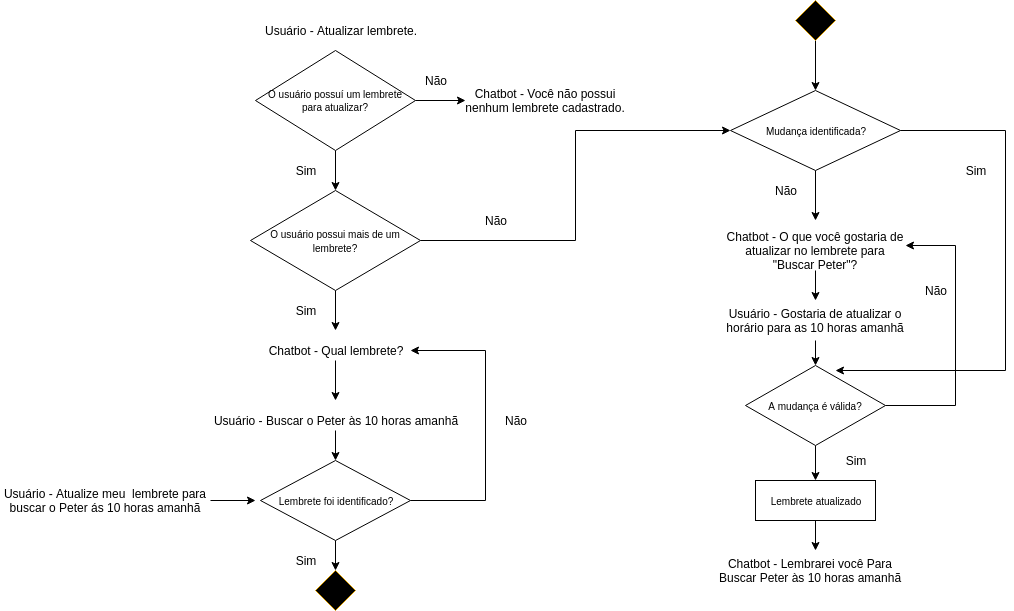
\includegraphics[width=0.9\linewidth]{src/imagens/Chatbot.png}
\caption{\textit{Chatbot flowchart}} Fonte:~\cite{Samer}
\label{cap:01:fig:fluxograma}
\end{figure}

Outra característica importante nesse tipo de \textit{chatbots}, é que eles não precisam necessariamente compreender a linguagem humana para executarem suas tarefas~\cite{Juliano}.

\subsection{\textit{Chatbots} de domínio amplo}\label{cap:02:sec:01:sub:02:bot-dominio}

Já os \textit{chatbots} de domínio amplo utilizam de recursos mais avançados de Inteligência Artificial (\abrv[IA - Inteligência Artificial]{IA}), são capazes de compreender o que o usuário solicita e podem relacionar-se a qualquer área de domínio de conhecimento~\cite{Juliano}. 
Na maior parte do tempo, o atendimento realizado por esse tipo de \textit{chatbots}, procura simular a conversação em linguagem humana.
Em outras palavras, um dos objetivos principais é responder perguntas de forma que os usuários tenham a impressão de estarem conversando com outra pessoa e não com um programa de computador.
Para isso, são utilizadas técnicas de Aprendizagem de Máquina (\textit{Machine Learning}) ou de Processamento de Linguagem Natural (\textit{Natural Language Processing})~\cite{Falaki}. 
Assim, o \textit{chatbot} é treinado com base nas interações dos usuários e consegue aprender com elas, se tornando mais inteligente e preciso ao decorrer deste processo.

As Assistentes Virtuais Inteligentes (\abrv[AVIs - Assistentes Virtuais Inteligentes]{AVIs}) são um dos exemplos de \textit{chatbots} desse tipo. 
As AVIs são uma das principais tendências de soluções para otimizar o relacionamento entre empresas e consumidores~\cite{DDS}. 
Por meio de mecanismos de Inteligência Artificial, elas aprendem a partir das interações com o consumidor e, com isso, melhoram o seu repertório. 
Assim, são capazes de entender as necessidades do cliente e auxiliá-los da devida maneira na resolução de seus problemas.

\section{Inteligência artificial para \textit{chatbots}}\label{cap:02:sec:02:ia}

\subsection{Aprendizado de máquina}\label{cap:02:sec:02:sub:machine-learning}

De maneira simplificada, Aprendizagem de máquina é a prática de usar algoritmos para coletar dados, aprender com eles, e então fazer uma determinação ou predição sobre alguma atividade específica~\cite{SimpleML}. Assim ao invés de implementar as rotinas de software propriamente ditas, com um conjunto específico de instruções para completar uma tarefa em particular, a máquina é “treinada” usando uma quantidade grande de dados e algoritmos que dão e ela a habilidade de aprender como executar a tarefa. De maneira mais técnica, é um método de análise de dados que automatiza a construção de modelos analíticos~\cite{SASML}. Se baseia na ideia de que sistemas podem aprender com dados, identificar padrões e tomar decisões com o mínimo de intervenção humana.

Existem vários serviços que fornecem e facilitam o uso de tecnologias de aprendizagem de máquina, um deles, por exemplo, é a Amazon Machine Learning.
O Amazon Machine Learning oferece ferramentas e assistentes de visualização que orientam o desenvolvedor durante o processo de criação de modelos de aprendizado de máquina, sem necessidade de aprender tecnologias e algoritmos complexos para o desenvolvimento de tal. 


\subsection{Processamento de Linguagem Natural}\label{cap:02:sec:02:sub:pln}

O Processamento de Linguagem Natural (\abrv[PLN - Processamento de Linguagem Natural]{PLN}) é a subárea da IA que estuda a capacidade e as limitações de uma máquina em entender a linguagem dos seres humanos~\cite{PLN1}.
Alguns dos objetivo do PLN é fornecer aos computadores a capacidade de  reconhecer o contexto, fazer análise sintática, semântica, léxica e morfológica, criar resumos, extrair informação, interpretar os sentidos, analisar sentimentos e até aprender conceitos com os textos processados~\cite{PLN1}.

Um dos métodos utilizados do PLN para o desenvolvimento de \textit{chatbots} é transformar uma sentença textual (dado) em informação (intenção e entidades)~\cite{Anatomy}. Em outras palavras, as intenções expressam funcionalidades, entidades expressam parâmetros para a execução de uma funcionalidade. Essas entidades precisam ser cadastradas, de forma a servir à base de conhecimento do PLN. Depois criamos as intenções, onde determinamos frases e sentenças que usarão essas entidades para expressar essas intenções. Assim, de modo simplório, o PLN passa a conseguir interpretar textos completos, textos simples e até mesmo incompletos.

Atualmente, existem vários serviços que dão suporte para a criação de PLN, um desses exemplos é o Wit.ia. Wit.ai é uma plataforma de desenvolvimento de PLN gratuita que transforma a linguagem natural (fala ou escrita) em dados estruturados. Um dos principais motivos para o uso do Wit.ai é por sua simplicidade no processo de criação de aplicativos e dispositivos com os quais as pessoas podem conversar, nesse contexto, na criação de \textit{chatbots}. Com isso, se abstrai a necessidade de aprender todo o processo de desenvolvimento de algoritmos de PLN.


\section{\textit{Chatbots} em plataformas de mensagens instantâneas}\label{cap:02:sec:03:sub:chatbotsmessenger}

Um mensageiro instantâneo consiste em um software que permite que diferentes usuários troquem mensagens, geralmente por escrito, em tempo real. 
Esses mensageiros instantâneos podem possuir alguns recursos adicionais como o envio de arquivos, conversas de áudio, conversas coletivas e até video conferências.
O termo mensageiro instantâneo, no entanto, encontra-se em desuso, sendo agora chamado com mais frequência por plataformas de mensagens instantâneas, ou simplesmente por \textit{messengers}. Podemos citar alguns \textit{messengers} como exemplo, tais como o Whatsapp, Telegram, WeChat, Slack, Facebook Messenger, entre outros.

No que se diz respeito à criação de \textit{chatbots}, alguns desses \textit{messengers} oferecem ferramentas e suporte, sob licenças especificas, para o desenvolvimento em sua plataforma, por meio de \textit{Application Programming Interfaces} (APIs).
Dentre os \textit{messengers}, um dos mais famosos por possuírem tais funcionalidades, é o Telegram.
O Telegram foi lançado em 2015 e possuí cerca de 100 milhões de usuários ativos mensais~\cite{IMaster}, 
É válido ressaltar também, os seus recursos avançados em questão de segurança e criptografia.
O Telegram oferece suporte para desenvolvimento de \textit{chatbots} desde 2015, por meio de sua API baseada no protocolo \abrv[HTTP - Hypertext Transfer Protocol]{HTTP} (Hypertext Transfer Protocol).


\section{Projetando \textit{chatbots}}\label{cap:02:sec:05:projeto}

Como sistemas computacionais são construídos para terem utilidade no mundo real, modelar o domínio de aplicação é uma atividade de suma importância.
A partir dessa atividade, pode se compreender a necessidade do sistema a ser construído e também definir os requisitos que tornam o sistema útil~\cite{ReqJair}. 
Pelo fato do \textit{chatbot} também se tratar de um produto digital, algumas práticas e estudos também devem ser realizados em seu processo de criação. Algumas dessas pŕaticas envolvem a análise e especificação dos requisitos e a elaboração dos diálogos que farão parte do repertório de um \textit{chatbot}.

\subsection{Análise e especificação dos requisitos}

De acordo com \alusao{ReqJair} a análise e especificação de requisitos de software envolve as atividades de determinar os objetivos de um software e as restrições associadas a ele.
\alusao{ReqJair} diz que a análise é o processo de observação e levantamento dos elementos do domínio no qual o sistema será introduzido. Deve-se identificar  as pessoas, atividades, informações do domínio para que se possa decidir o que deverá ser informatizado ou não.
Já a especificação é a descrição sistemática e abstrata do que o software deve fazer, a partir daquilo que foi analisado.

\subsubsection{Classificação de requisitos}\label{cap:02:sec:05:projeto:classificacao-requisitos}

\alusao{Sommerville} estabelece que os requisitos de um sistema são as descrições do que o sistema deve fazer, os serviços que oferece e as restrições a seu funcionamento.
Esses requisitos refletem as necessidades dos clientes para um sistema que serve a uma finalidade determinada, como controlar um dispositivo, efetuar um pedido ou encontrar informações.
É válido ressaltar que os requisitos de software são frequentemente classificados como requisitos funcionais e requisitos não funcionais.

Os requisitos funcionais de um sistema descrevem o que ele deve fazer.
Eles dependem do tipo de software a ser desenvolvido, de quem são seus possíveis usuários e da abordagem geral adotada pela organização ao escrever os requisitos~\cite{Sommerville}.
Quando expressos como requisitos de usuário, os requisitos funcionais são normalmente descritos de forma abstrata, para serem compreendidos pelos usuários do sistema.\label{texto:requisito_funcional}

Já os requisitos não funcionais, como o nome sugere, são requisitos que não estão diretamente relacionados com os serviços específicos oferecidos pelo sistema a seus usuários~\cite{Sommerville}.
Eles podem estar relacionados às propriedades emergentes do sistema, como confiabilidade, tempo de resposta, integridade, disponibilidade, ocupação de área entre outros.\label{texto:requisito_nao_funcional}

\subsection{Especificando requisitos utilizando casos de uso}

De acordo com \alusao{ReqJair} um caso de uso especifica o comportamento do sistema a ser desenvolvido sem, no entanto, especificar como este comportamento será implementado.
Os comportamentos descrevem as funções da aplicação que caracterizam a funcionalidade do sistema.
Um caso de uso representa o que o sistema faz e não como o sistema faz, proporcionando uma visão externa e não interna do sistema. Cada caso de uso define um requisito funcional do sistema~\cite{ReqJair}.

O caso de uso descreve um conjunto de sequências de ações que o sistema desempenha para produzir um resultado esperado pelo usuário.
Cada sequência representa a interação de entidades externas e o sistema~\cite{ReqJair}.
Estas entidades são chamadas de atores e que podem ser usuários ou outros sistemas.
No caso de usuários, um ator representa na verdade uma função de usuários. Para isso, normalmente se utiliza da notação UML como linguagem de especificação para representar os casos de uso. Na Figura~\ref{cap:02:fig:caso-de-uso-exemplo}, segue um exemplo de especificação de casos de uso utilizando a notação UML de um sistema de vendas.\label{texto:especificando-com-casos-de-uso}

\begin{figure}[htb!]
\centering
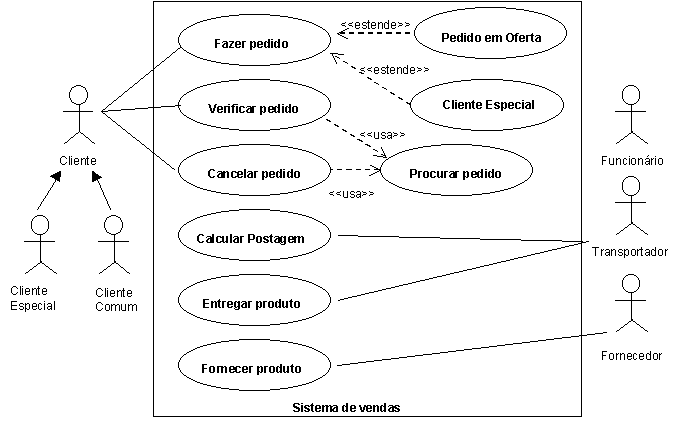
\includegraphics[width=0.7\linewidth]{src/imagens/casosd2.png}
\caption{Caso de uso - Sistema de Vendas} Fonte:~\cite{ReqJair2}
\label{cap:02:fig:caso-de-uso-exemplo}
\end{figure}

\subsection{Elaboração dos diálogos de um \textit{chatbot} a partir de cenários}\label{texto:elaborando-dialogos}

Para a elaboração dos diálogos que irão fazer parte do repertório de um \textit{chatbot}, uma técnica utilizada para a sua modelagem e especificação se dá pelo uso dos cenários.
\alusao{ReqJair} diz que cenários consistem de uma coleção de narrativas de situações no domínio que favorecem o levantamento de informações, a identificação de problemas e a antecipação das soluções.
Cenários são uma maneira de representar, no contexto de \textit{chatbots}, os diálogos e interações e as possibilidades que podem surgir a partir destes. Abaixo, um exemplo de cenário que simula o diálogo entre uma atendente e um cliente que deseja consultar seu histórico de compras:


\begin{itemize}
    \item \textbf{Suposição inicial:}
    
    O cliente informa que deseja consultar o seu histórico de compras; a atendente pergunta suas informações pessoais (nome e CPF); o cliente informa seus dados; a atendente faz uma consulta com base nos dados adquiridos; a atendente exibe o histórico de compras do cliente.
    
    \begin{enumerate}
        \item \textbf{Cliente}: Gostaria de consultar meu histórico de compras, por favor.
        \item \textbf{Atendente}: O senhor poderia me informar o seu nome completo e os três últimos dígitos do seu CPF?
        \item \textbf{Cliente}: Claro. Meu nome é Custódio de Almeida, e os três últimos dígitos do meu CPF são 186.
        \item \textbf{Atendente}: Um instante, por favor.
        \item \textbf{Atendente}: O histórico do senhor é o seguinte: \\
        Dia: 20/02/2017 - 1 Tênis branco da marca X, 2 camisetas rosas da marca Y.\\
        Dia: 25/02/2017 - 2 shorts amarelos da marca Z.
        \ldots
    \end{enumerate}
    
    \item \textbf{O que pode dar errado:}
    
    As informações fornecidas pelo usuário não conferem com as cadastradas no banco de dados. A atendente informa o usuário que os dados informados não são válidos e pede para que ele tente novamente.
    
    \begin{enumerate}
        \item \textbf{Atendente}: Me desculpe, mas parece que os dados informados não conferem. Você poderia tentar novamente?
        \item \textbf{Cliente}: Certo. Tente os seguintes dados dessa vez \ldots
    \end{enumerate}
    
    O usuário nunca efetuou uma compra no estabelecimento. A atendente informa que o usuário não tem nenhuma compra na loja e informa as promoções disponíveis.
    
    \begin{enumerate}
        \item \textbf{Atendente}: Me desculpe, mas parece que o senhor não possui nenhuma compra em nossa loja.
        \item \textbf{Cliente}: Tudo bem, então.
        \item \textbf{Atendente}: Caso seja do seu interesse, nós estamos com uma promoção de 30\% de desconto na compra de qualquer camiseta da marca X. Você gostaria de dar uma olhada? \ldots
    \end{enumerate}
    
    \item \textbf{Estado do sistema na conclusão:}
    
    Após exibir o histórico do cliente, a atendente irá perguntar se o ele deseja mais alguma coisa.
    
    \begin{enumerate}
        \item \textbf{Atendente}: Esse é todo o seu histórico de compras em nossa loja. Existe mais alguma coisa em que eu possa lhe ajudar?
        \ldots
    \end{enumerate}
    
    
\end{itemize}


\section{Desenvolvimento de \textit{chatbots}}\label{chatbot:dev}

No desenvolvimento de \textit{chatbots}, pode-se dizer que existem duas maneiras para a sua criação: utilizando ferramentas de plataformas de \textit{chatbots} ou não. Para melhor explicar a vantagens e desvantagens de cada modo, nas subseções abaixo, estes serão detalhados.

\subsection{Utilizando plataformas de \textit{chatbots}}\label{chatbot:dev:plat}

A plataformas de \textit{chatbots} são sistemas que oferecem serviços para facilitar a criação de \textit{chatbots} e sua integração com os  \textit{messengers}.
Basicamente, essas plataformas abstraem a necessidade de programar rotinas de códigos complexas, já oferecem recursos ou serviços de IA embutidos e também a tradução da aplicação, aonde o \textit{chatbot} poderá ser exportado e integrado para os mais diversos \textit{messengers}.
O intuito dessas plataformas, é elevar a produtividade dos desenvolvedores responsáveis pela criação do \textit{chatbot}.
Assim, ao facilitar o processo de criação, abstraindo várias etapas complexas e trabalhosas, eles serão capazes de desenvolverem o \textit{chatbot} em menos tempo.
Como exemplo dessas plataformas de \textit{chatbots}, podemos citar a Microsoft Bot Plataform, ChatScript, Pandorabots, Facebook Bots for Messenger, BLIP, entre outros.

Porém, para que possam se utilizar dos recursos mais avançados dessas plataformas, as empresas ou desenvolvedores contratantes devem efetuar os pagamentos, que podem variar de acordo com o tipo de serviço solicitado, podendo estes serviços serem mais caros de acordo com o número de usuários simultâneos que o \textit{chatbot} poderá atender, até, em questões de utilização de recursos mais sofisticados e personalizados para agilizar no desenvolvimento dos \textit{chatbots}. 


\subsection{Não utilizando plataformas de \textit{chatbots}}\label{chatbot:dev:nplat}

Caso o desenvolvedor opte pela não utilização dessas plataformas de \textit{chatbots}, ele poderá customizar a sua aplicação utilizando as tecnologias, ferramentas e serviços que lhe bem convir.
Por exemplo, ele poderá escolher desde de uma linguagem de programação específica até qual serviço de IA (caso seja um \textit{chatbot} de domínio amplo) que ele irá utilizar no projeto.
Como dito na seção \ref{cap:02:sec:03:sub:chatbotsmessenger}, muitos \textit{messengers} oferecem suporte e serviços, por meio de suas APIs, que facilitam o processo de desenvolvimento e integração do \textit{chatbot} em sua plataforma.
Assim, o desenvolvedor poderá avaliar dentre os serviços oferecidos por esses \textit{messengers} e escolher qual lhe oferece mais benefícios.

É válido ressaltar a existência de bibliotecas que facilitam ainda mais o de desenvolvimento de \textit{chatbots}.
Essas, por sua vez, abstraem algumas etapas no processo de criação e integração dos \textit{chatbots} com os \textit{messengers}.
Podemos resumi-las em uma implementação real das regras de uma API de um \textit{messenger}, no contexto de \textit{chatbots}, elas oferecem uma interface mais simplificada para o seu desenvolvimento, utilizando alguma linguagem de programação específica, aonde se abstrai, por exemplo, a necessidade de programar rotinas que possibilitem a comunicação do \textit{chatbot}, via algum protocolo pré-determinado, com a API do \textit{messenger}.


  % Capitulo 3: Terceiro capítulo (arquivo Includes/Capitulo3.tex)
  \chapter{Desenvolvimento de EVA}

\section{Apresentação do projeto}

A EVA (EV.G Virtual Assistant) é um \textit{chatbot} de domínio amplo que será capaz de interagir com os alunos vinculados ao EV.G na medida de suas necessidades. Ela irá atender tais solicitações via mecanismo de conversação textual na plataforma de mensagens instantâneas chamada Telegram, no atendimento administrativo de uma secretaria acadêmica.

Por meio de EVA, os alunos vinculados ao EV.G poderão usufruir de várias funcionalidades. Eles irão gerenciar seus cursos visualizando o andamento das inscrições, terão acesso ao catálogo unificado, calendário de turmas, histórico escolar e também serão auxiliados no processo de emissão de certificado. Tudo por meio de um acesso único e simplificado.

\subsection{Especificação dos requisitos}

Como sistemas computacionais são construídos para terem utilidade no mundo real, modelar o domínio de aplicação é uma atividade extremamente importante. A partir dessa atividade, pode se compreender a necessidade e a importância do sistema a ser construído e também definir os requisitos que tornam o sistema útil.

De acordo com \cite{} requisitos são objetivos ou restrições estabelecidas por clientes e usuários do sistema que definem as diversas propriedades do sistema. Os requisitos  de software são, obviamente, aqueles dentre os requisitos de sistema que dizem respeito a propriedades do software.

Um conjunto de requisitos pode ser definido como uma condição ou capacidade necessária que o software deve possuir (1) para que o usuário possa resolver um problema ou atingir um objetivo ou (2) para atender as necessidades ou restrições da organização ou dos outros componentes do sistema.

\subsubsection{Requisitos funcionais}

Os requisitos funcionais são a descrição das diversas funções que clientes e usuários querem ou precisam que o software ofereça. Eles definem a funcionalidade desejada do software. O termo função é usado no sentido genérico de operação que pode ser realizada pelo sistema, seja através comandos dos usuários ou seja pela ocorrência de eventos internos ou externos ao sistema.


\subsubsection{Requisitos não-funcionais}

Requisitos não-funcionais são as qualidades globais de um software, como manutenibilidade, usabilidade, desempenho, custos e várias outras. Normalmente estes requisitos são descritos de maneira informal, de maneira controversa (por exemplo, o gerente quer segurança mas os usuários querem facilidade de uso) e são difíceis de validar.

\section{Arquitetura de EVA}

\subsection{Arquitetura da API}

\subsection{Arquitetura do \textit{chatbot}}

\section{Modelagem dos diálogos de EVA}

\subsection{Boas práticas}

\subsection{Desenvolvimento dos diálogos}

  % Capitulo 4: Quarto capítulo (arquivo Includes/Capitulo4.tex)
  \chapter{Apresentação de EVA}

Neste capítulo, serão apresentadas as principais funcionalidades de EVA, já em funcionamento, na plataforma de mensagens instantâneas Telegram. É válido salientar que por motivos de segurança e integridade, como estão sendo utilizados dados reais dos alunos vinculados a EV.G, em algumas figuras foram postas tarjas pretas sob informações que são consideradas pessoais do usuário.

\section{Boas-vindas}

Ao inicializar uma conversa com EVA, ela dará as boas-vindas e irá solicitar ao usuário que o mesmo se autentique, fornecendo o CPF ou o e-mail cadastrado na EV.G. Na Figura \ref{cap:04:fig:apresentacao-boas-vindas} é demonstrada tal situação.

\begin{figure}[htb!]
    \centering
    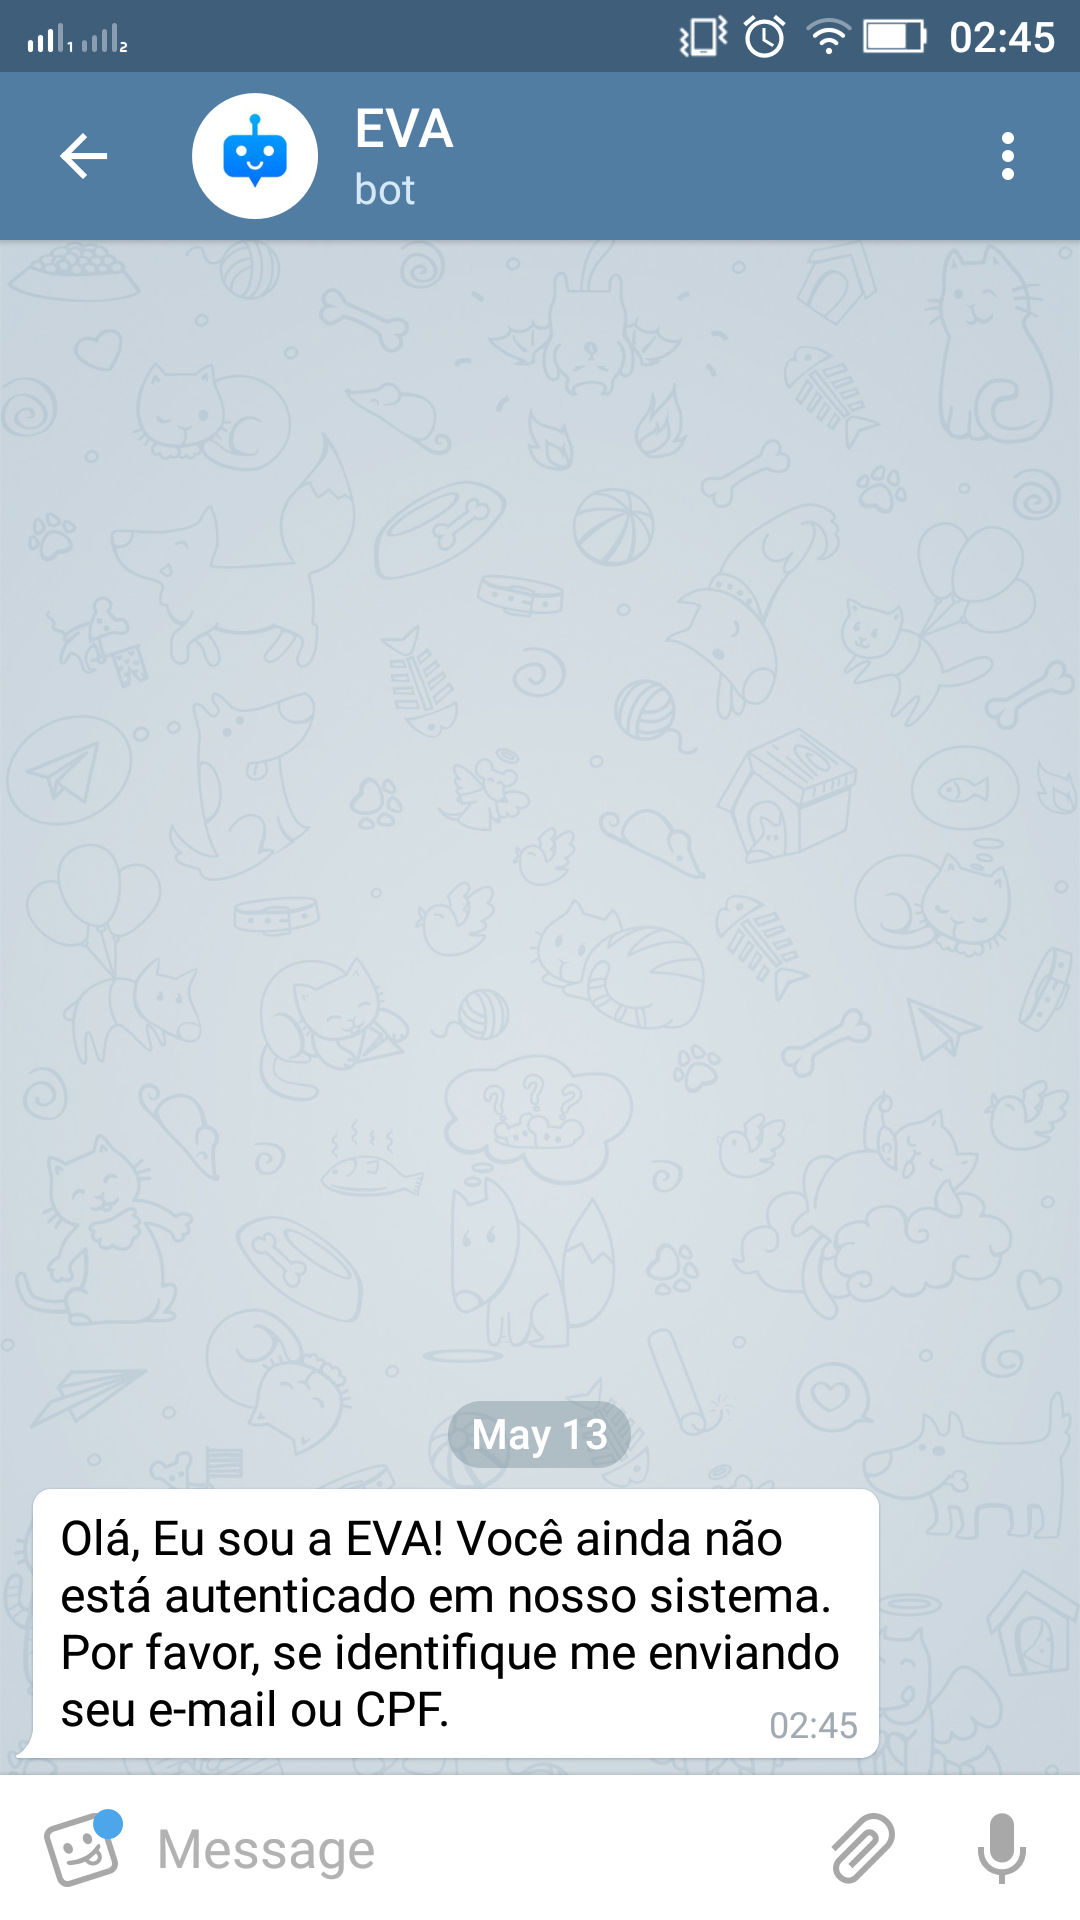
\includegraphics[width=0.2\linewidth]{src/imagens/apresentacao-boas-vindas.png}
    \caption{EVA - Boas-vindas} Fonte: Elaborado pelo autor (2018)
    \label{cap:04:fig:apresentacao-boas-vindas}
\end{figure}

\section{Autenticando}
O usuário poderá se autenticar para usufruir das funcionalidades mais sofisticadas de EVA. Para essa funcionalidade existem dois cenários possíveis: O de falha e o de sucesso na autenticação.

\subsection{Falha na autenticação}
Caso as credenciais fornecidas pelo usuário não estiverem corretas, EVA irá enviar uma mensagem dizendo que os dados não conferem e irá solicitar que o usuário informe o CPF ou o e-mail novamente. Se o usuário tentar se autenticar sem sucesso por três vezes consecutivas, o sistema irá bloqueá-lo por 24 horas e o \textit{chatbot} irá informar tal acontecimento ao usuário. Essas situações são apresentadas na Figura \ref{cap:04:fig:apresentacao-autenticação-falha}.

\begin{figure}[htb!]
    \centering
    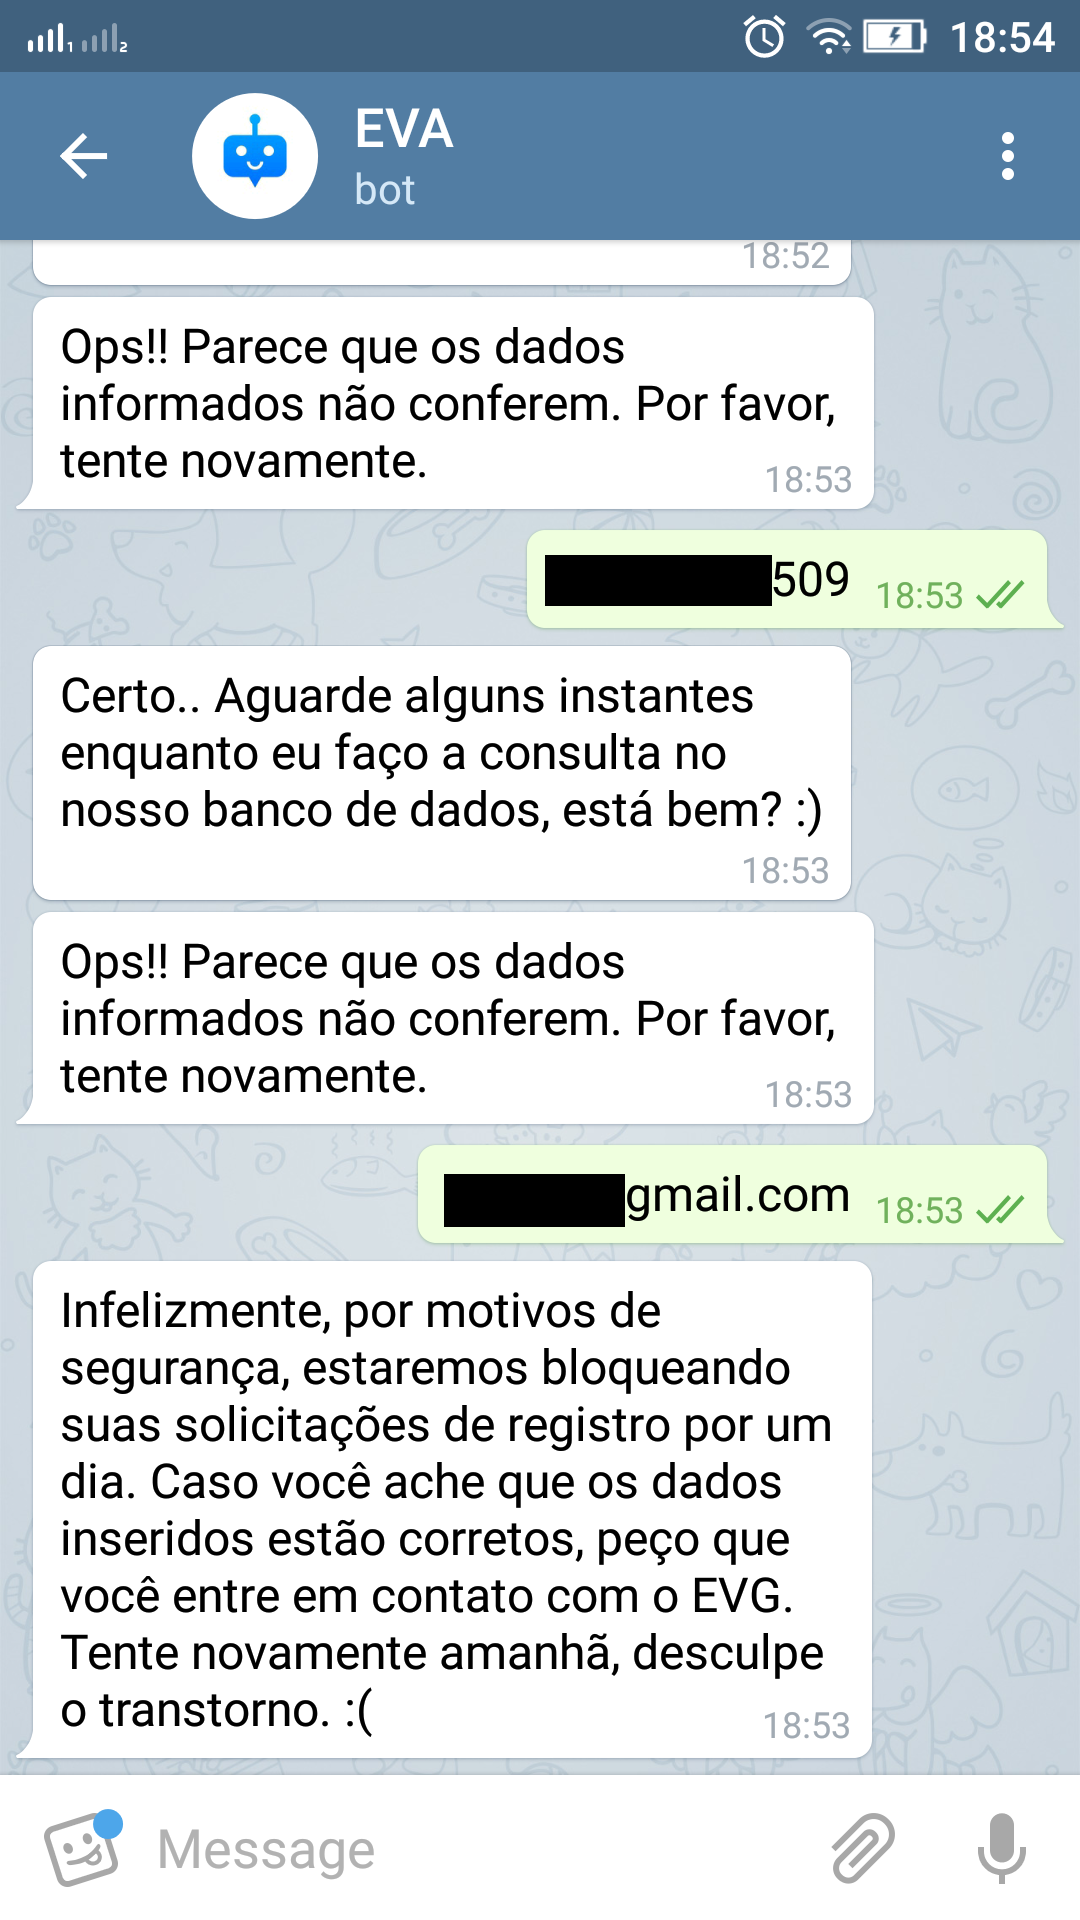
\includegraphics[width=0.2\linewidth]{src/imagens/apresentacao-autenticacao-falha.png}
    \caption{EVA - Bloqueio de usuário} Fonte: Elaborado pelo autor (2018)
    \label{cap:04:fig:apresentacao-autenticação-falha}
\end{figure}

\subsection{Sucesso na autenticação}
O aluno conseguiu se autenticar com sucesso no sistema e passará a ter acesso às funcionalidades mais sofisticadas de EVA. Na Figura \ref{cap:04:fig:apresentacao-autenticação-sucesso} este caso é apresentado.

\begin{figure}[htb!]
    \centering
    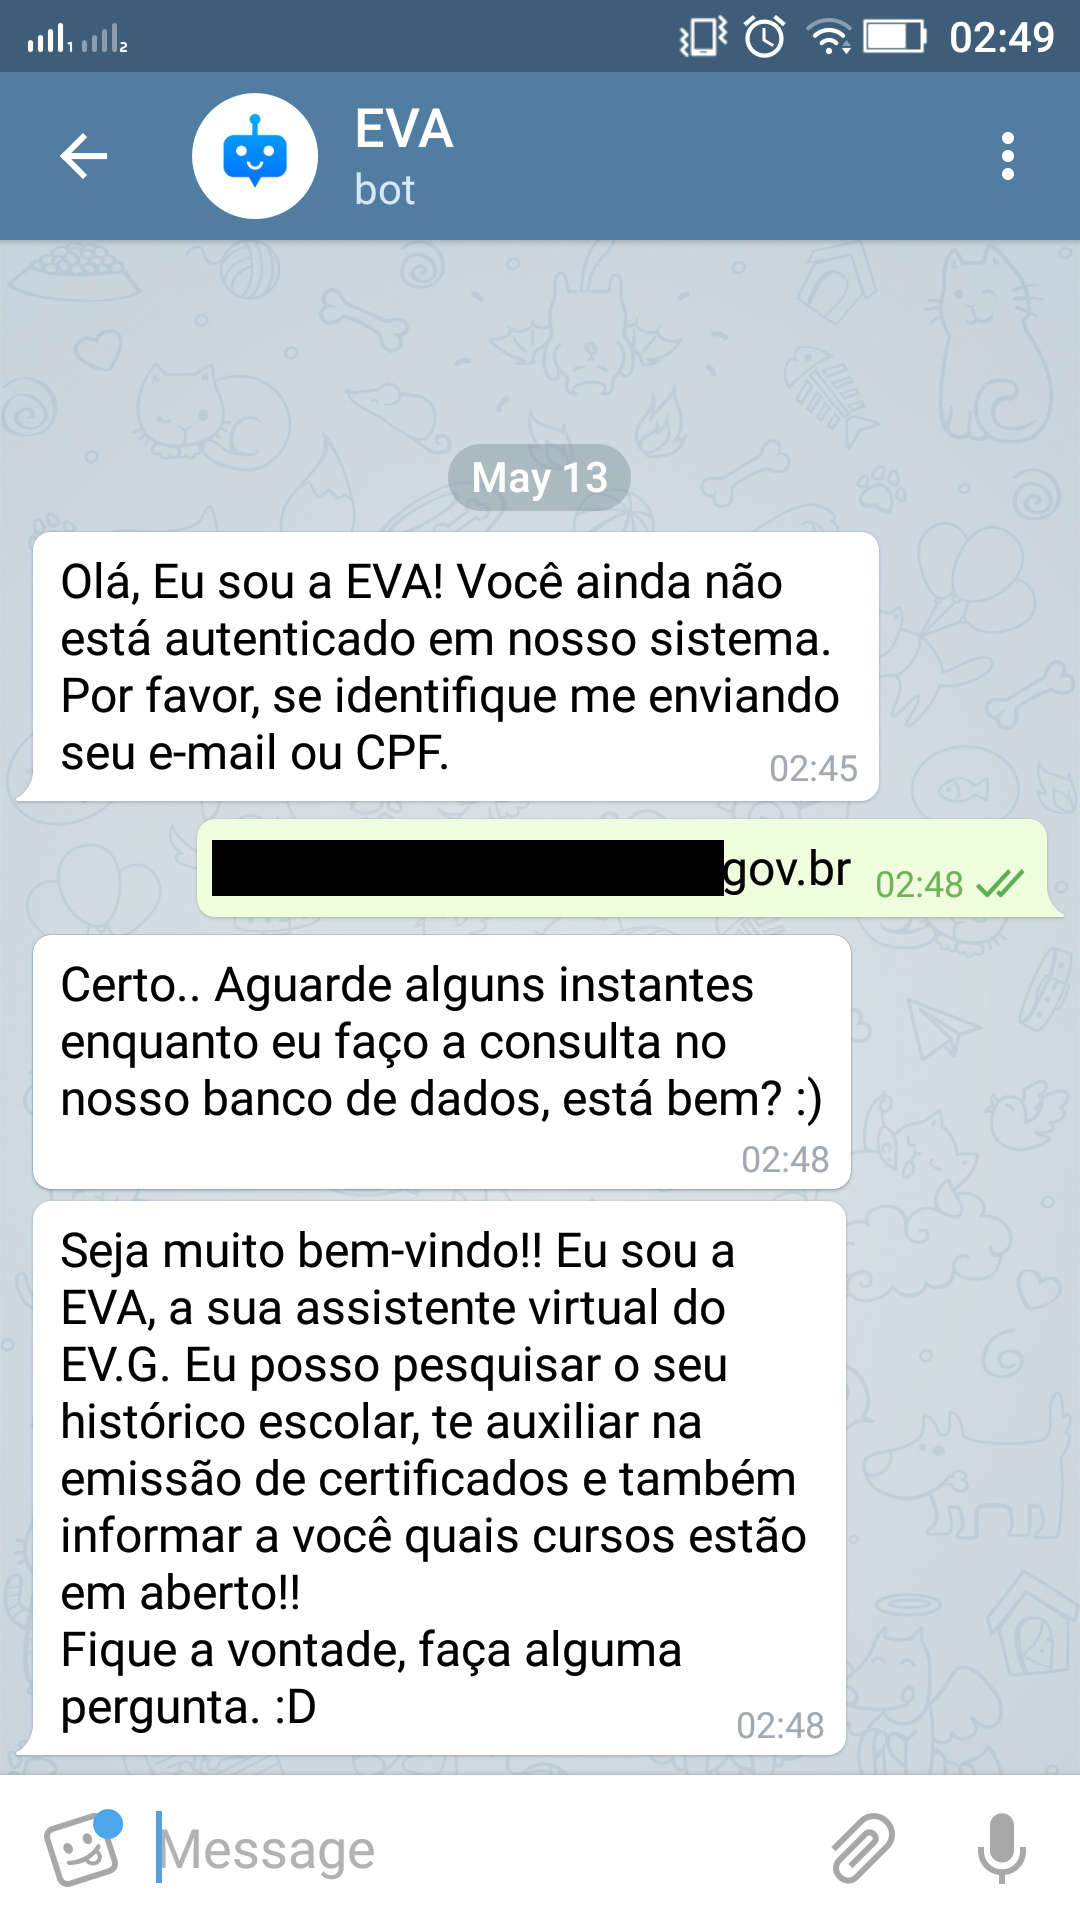
\includegraphics[width=0.2\linewidth]{src/imagens/apresentacao-autenticacao-sucesso.png}
    \caption{EVA - Autenticação realizada com sucesso} Fonte: Elaborado pelo autor (2018)
    \label{cap:04:fig:apresentacao-autenticação-sucesso}
\end{figure}

\section{Dialogando com EVA}

Por se tratar de um \textit{chatbot} de domínio amplo, EVA compreende algumas nuances nas mensagens enviadas por um aluno, compreendendo quais funcionalidades ele deseja utilizar e também sabendo quando um usuário está a cumprimentando, xingando e até mesmo quando recebe mensagens de afeto, como mostrada na Figura \ref{cap:04:fig:apresentacao-dialogos}.

\begin{figure}[htb!]
    \centering
    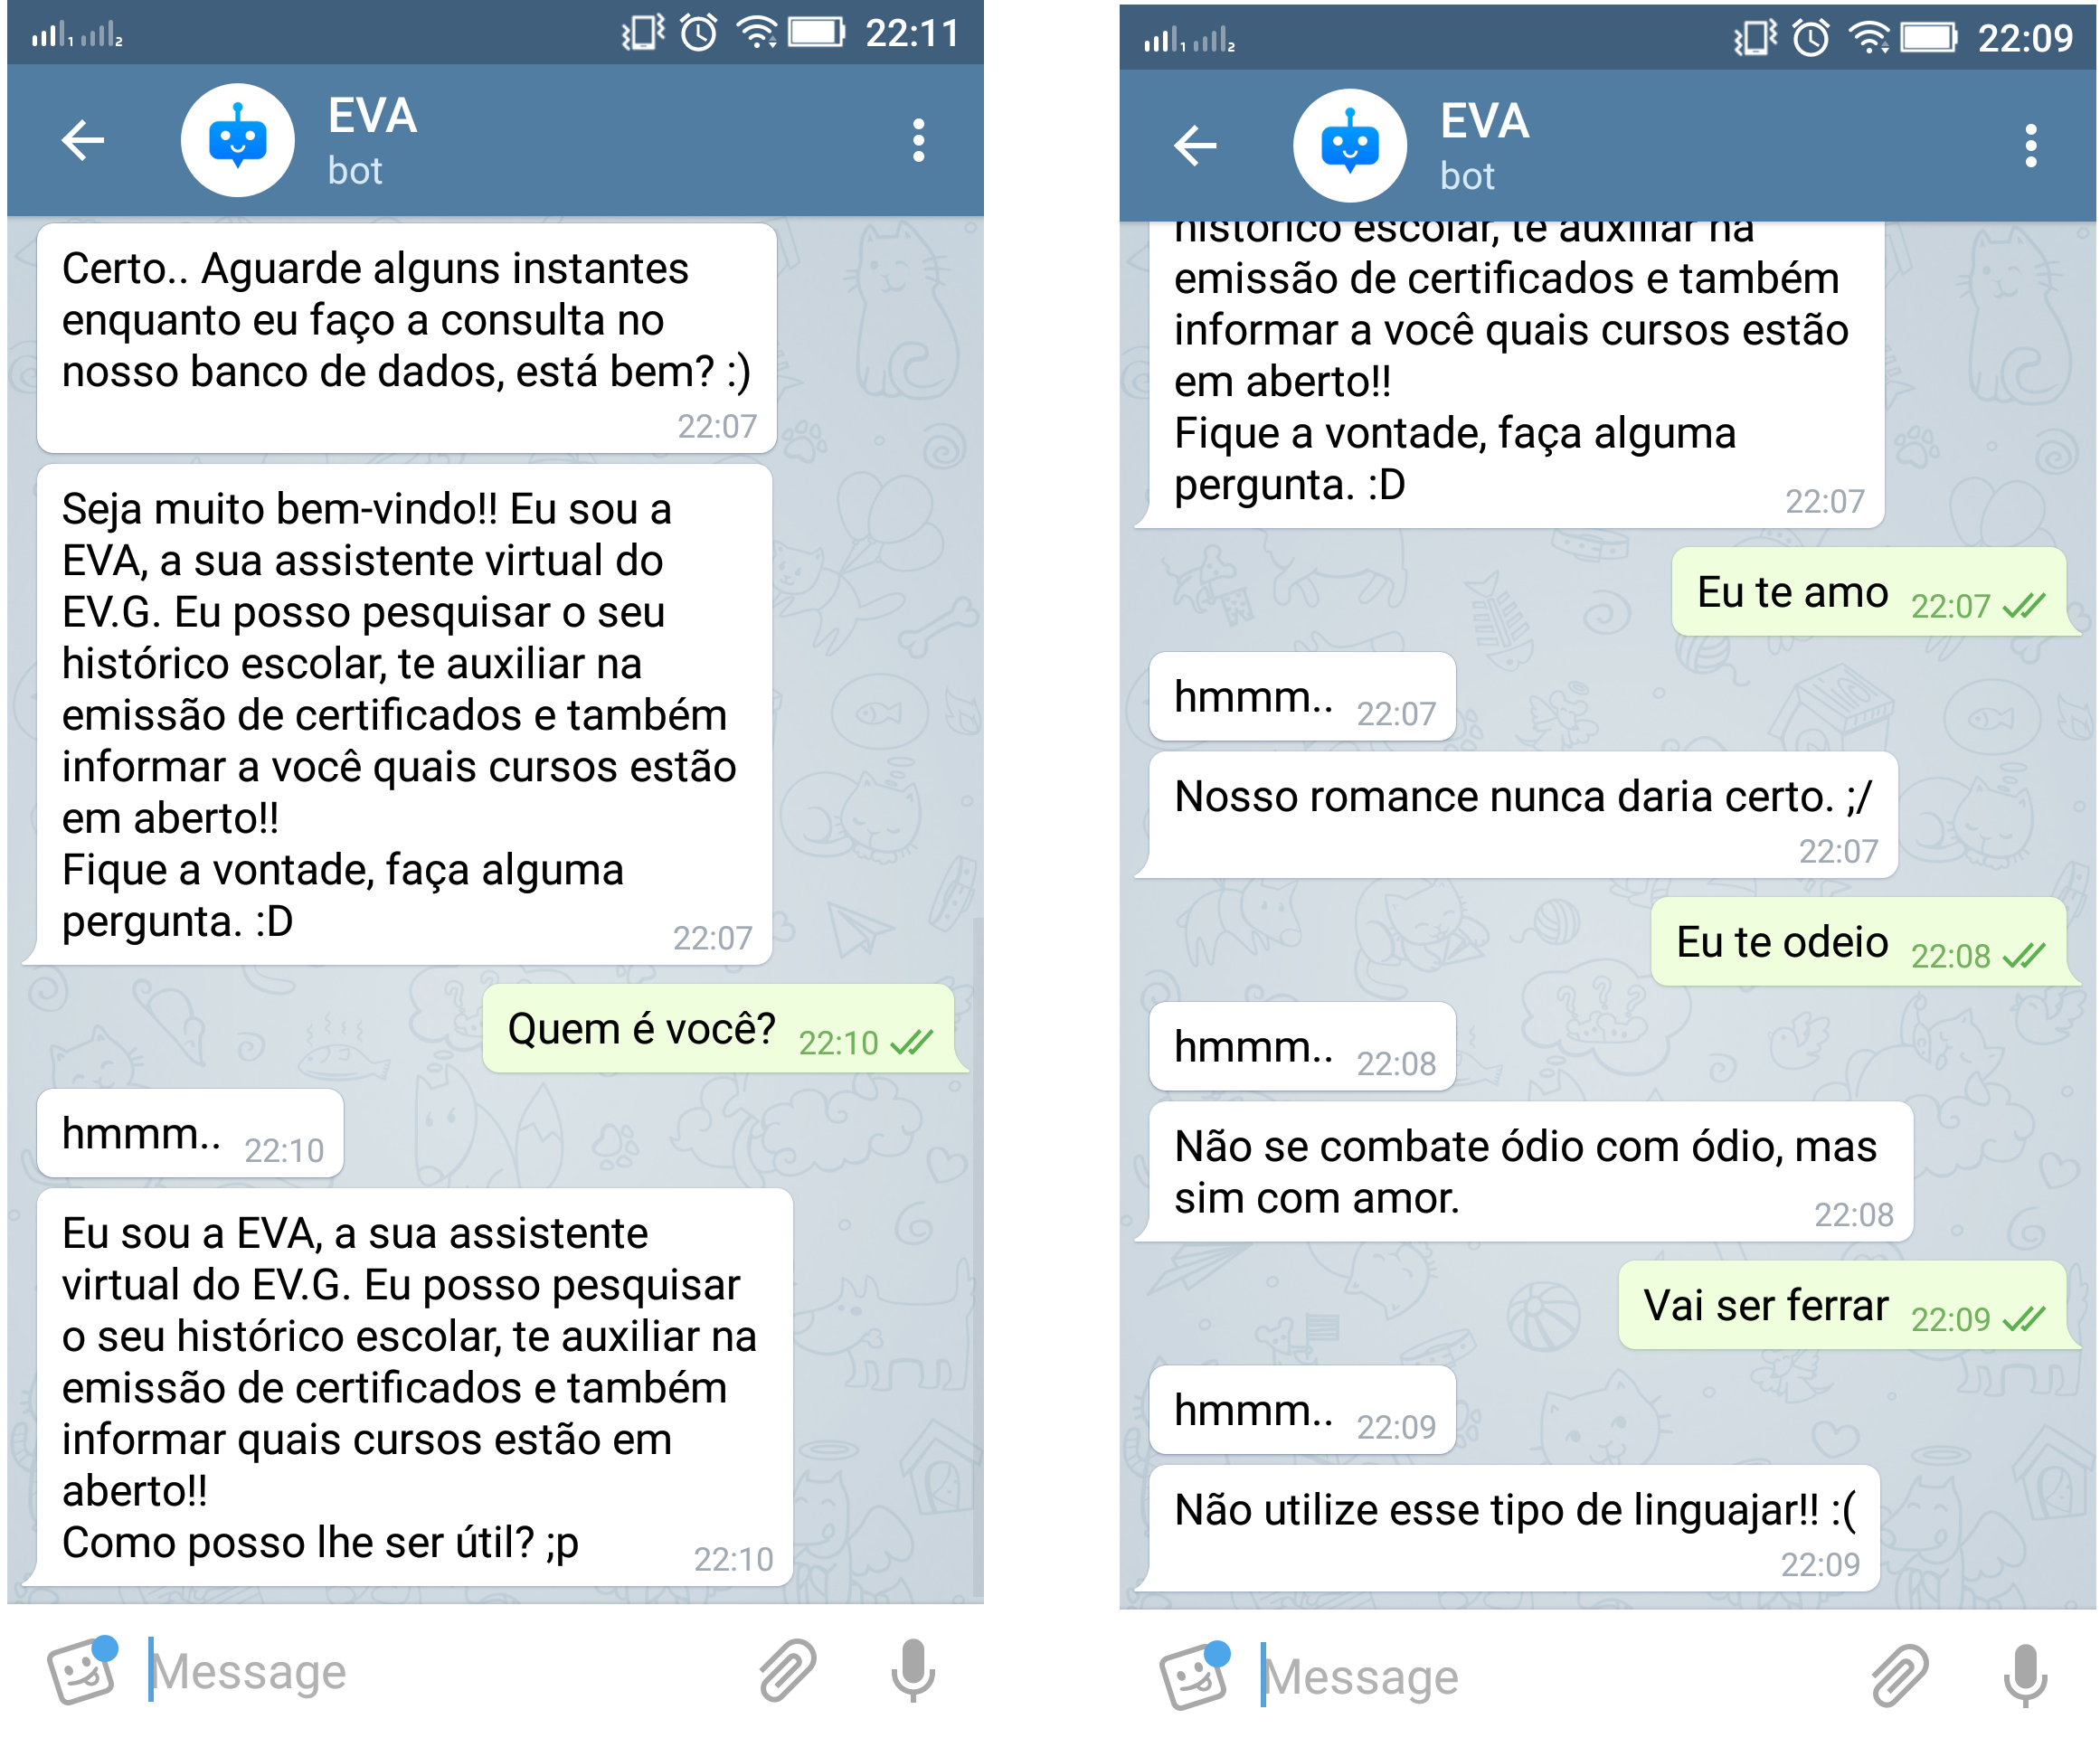
\includegraphics[width=0.4\linewidth]{src/imagens/apresentacao-dialogos.png}
    \caption{EVA - Dialogando} Fonte: Elaborado pelo autor (2018)
    \label{cap:04:fig:apresentacao-dialogos}
\end{figure}

\section{Visualizando o histórico escolar completo}

O aluno pode consultar o seu histórico escolar completo de maneira rápida e prática, como apresentado na Figura \ref{cap:04:fig:apresentacao-visualizar-historico}.

\begin{figure}[htb!]
    \centering
    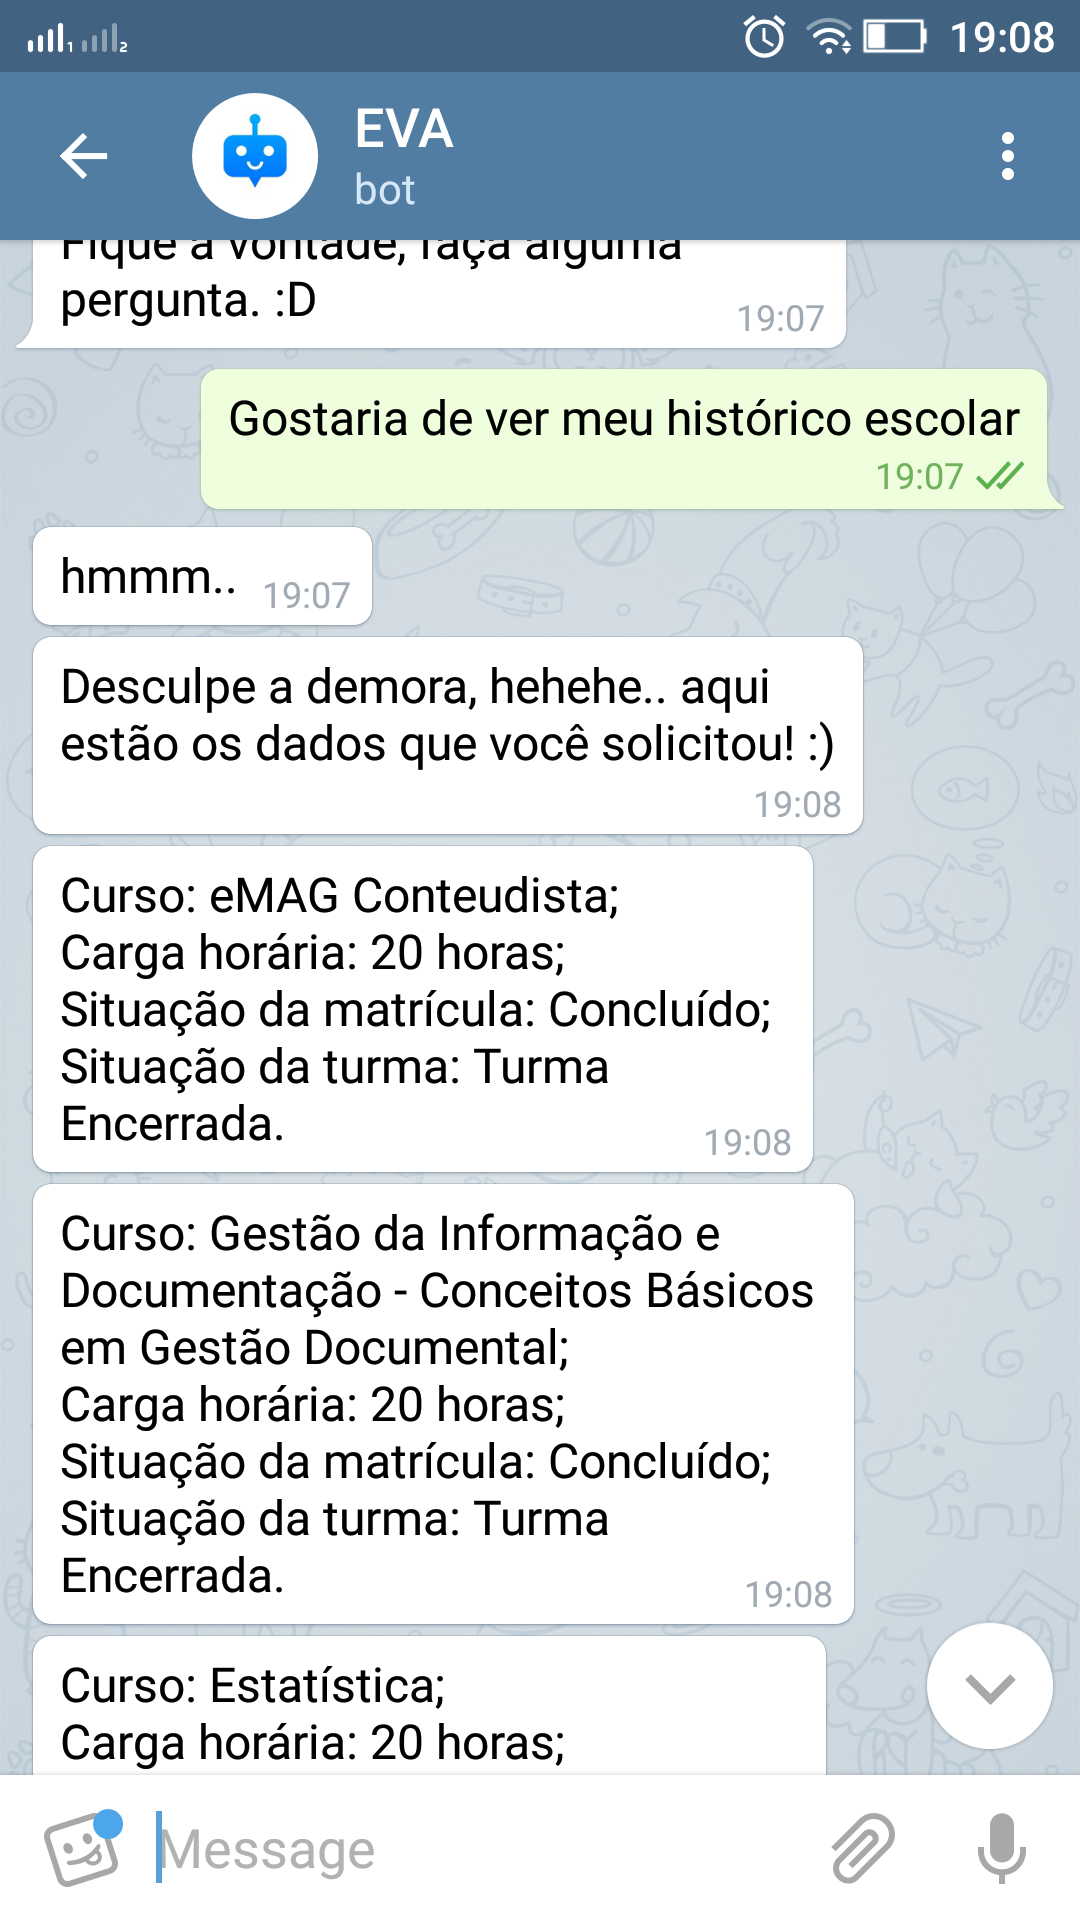
\includegraphics[width=0.2\linewidth]{src/imagens/apresentacao-visualizar-historico.png}
    \caption{EVA - Visualizando histórico escolar completo} Fonte: Elaborado pelo autor (2018)
    \label{cap:04:fig:apresentacao-visualizar-historico}
\end{figure}

\section{Auxiliando na emissão de certificados}

Se o aluno desejar, EVA pode auxiliá-lo na emissão de certificados dos cursos concluídos por ele, como exibido na Figura \ref{cap:04:fig:apresentacao-auxilio-certificados}.

\begin{figure}[htb!]
    \centering
    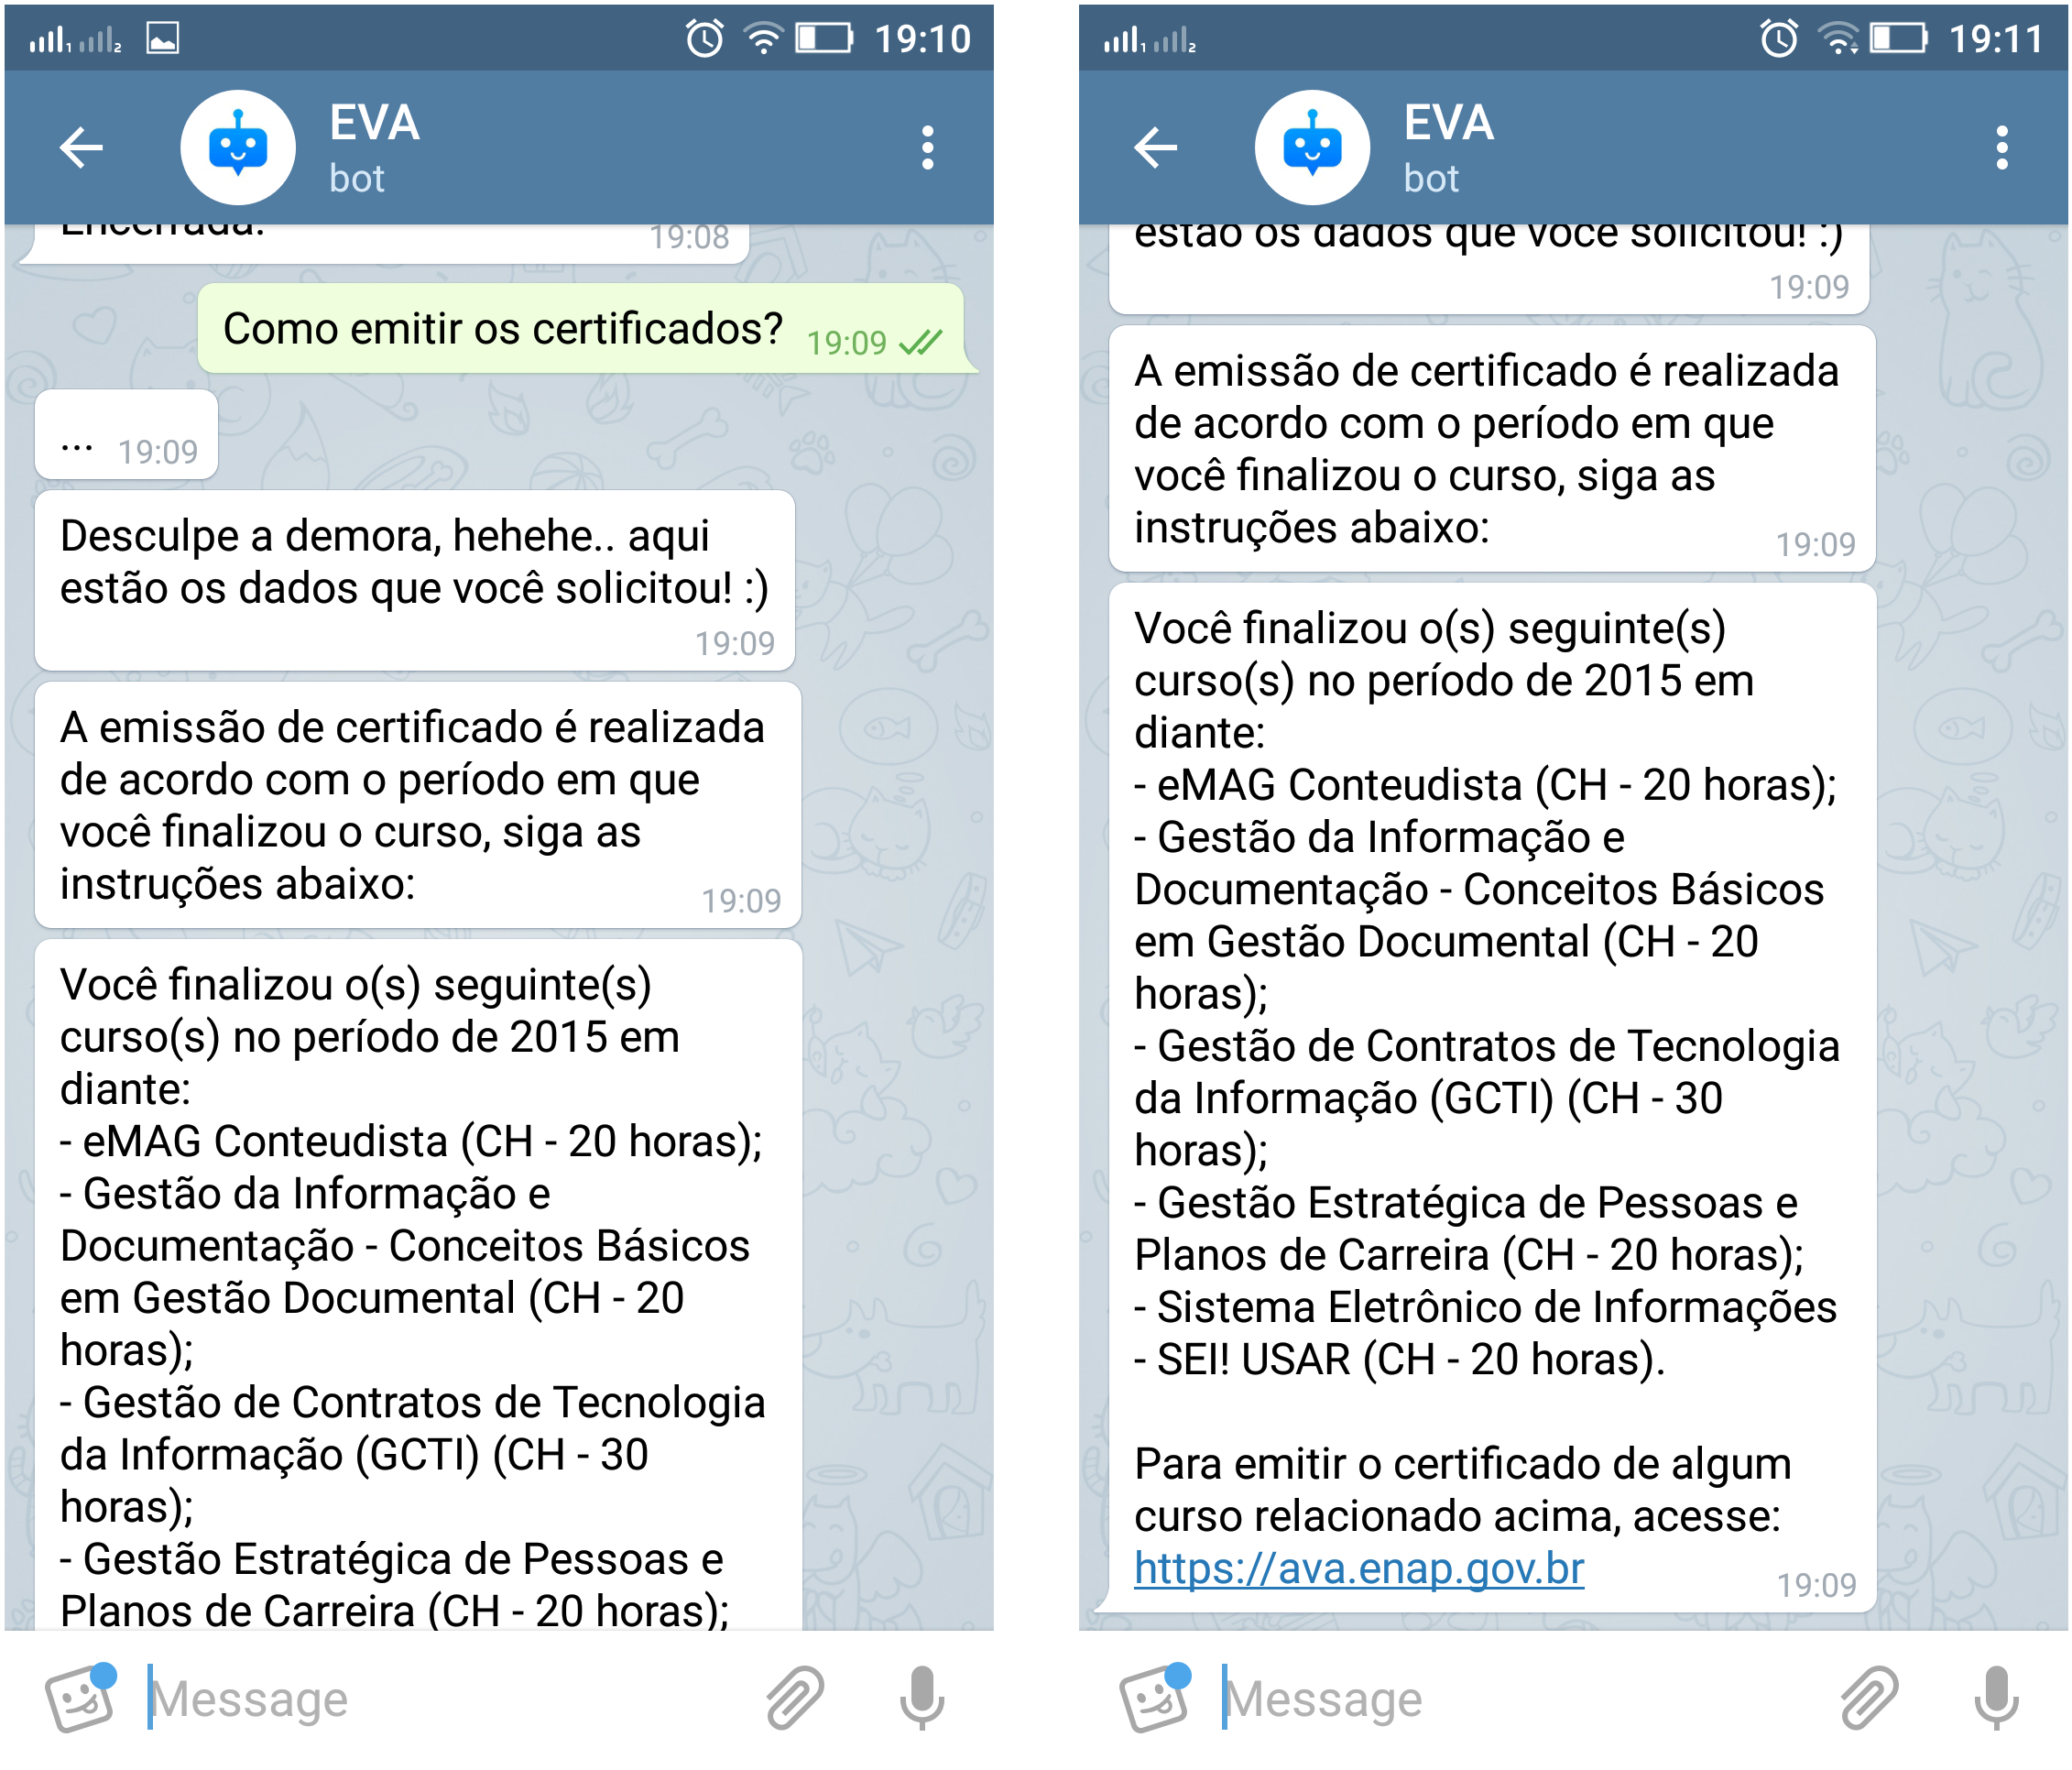
\includegraphics[width=0.4\linewidth]{src/imagens/apresentacao-auxilio-certificados.png}
    \caption{EVA - Auxiliando na emissão de certificados} Fonte: Elaborado pelo autor (2018)
    \label{cap:04:fig:apresentacao-auxilio-certificados}
\end{figure}

\section{Visualizando inscrições de cursos em aberto}

Caso o aluno esteja em dúvida sobre quais inscrições de cursos estão em aberto, com uma mensagem de texto ele terá acesso a essas informações, como apresentado na Figura \ref{cap:04:fig:apresentacao-inscricoes-aberto}.

\begin{figure}[htb!]
    \centering
    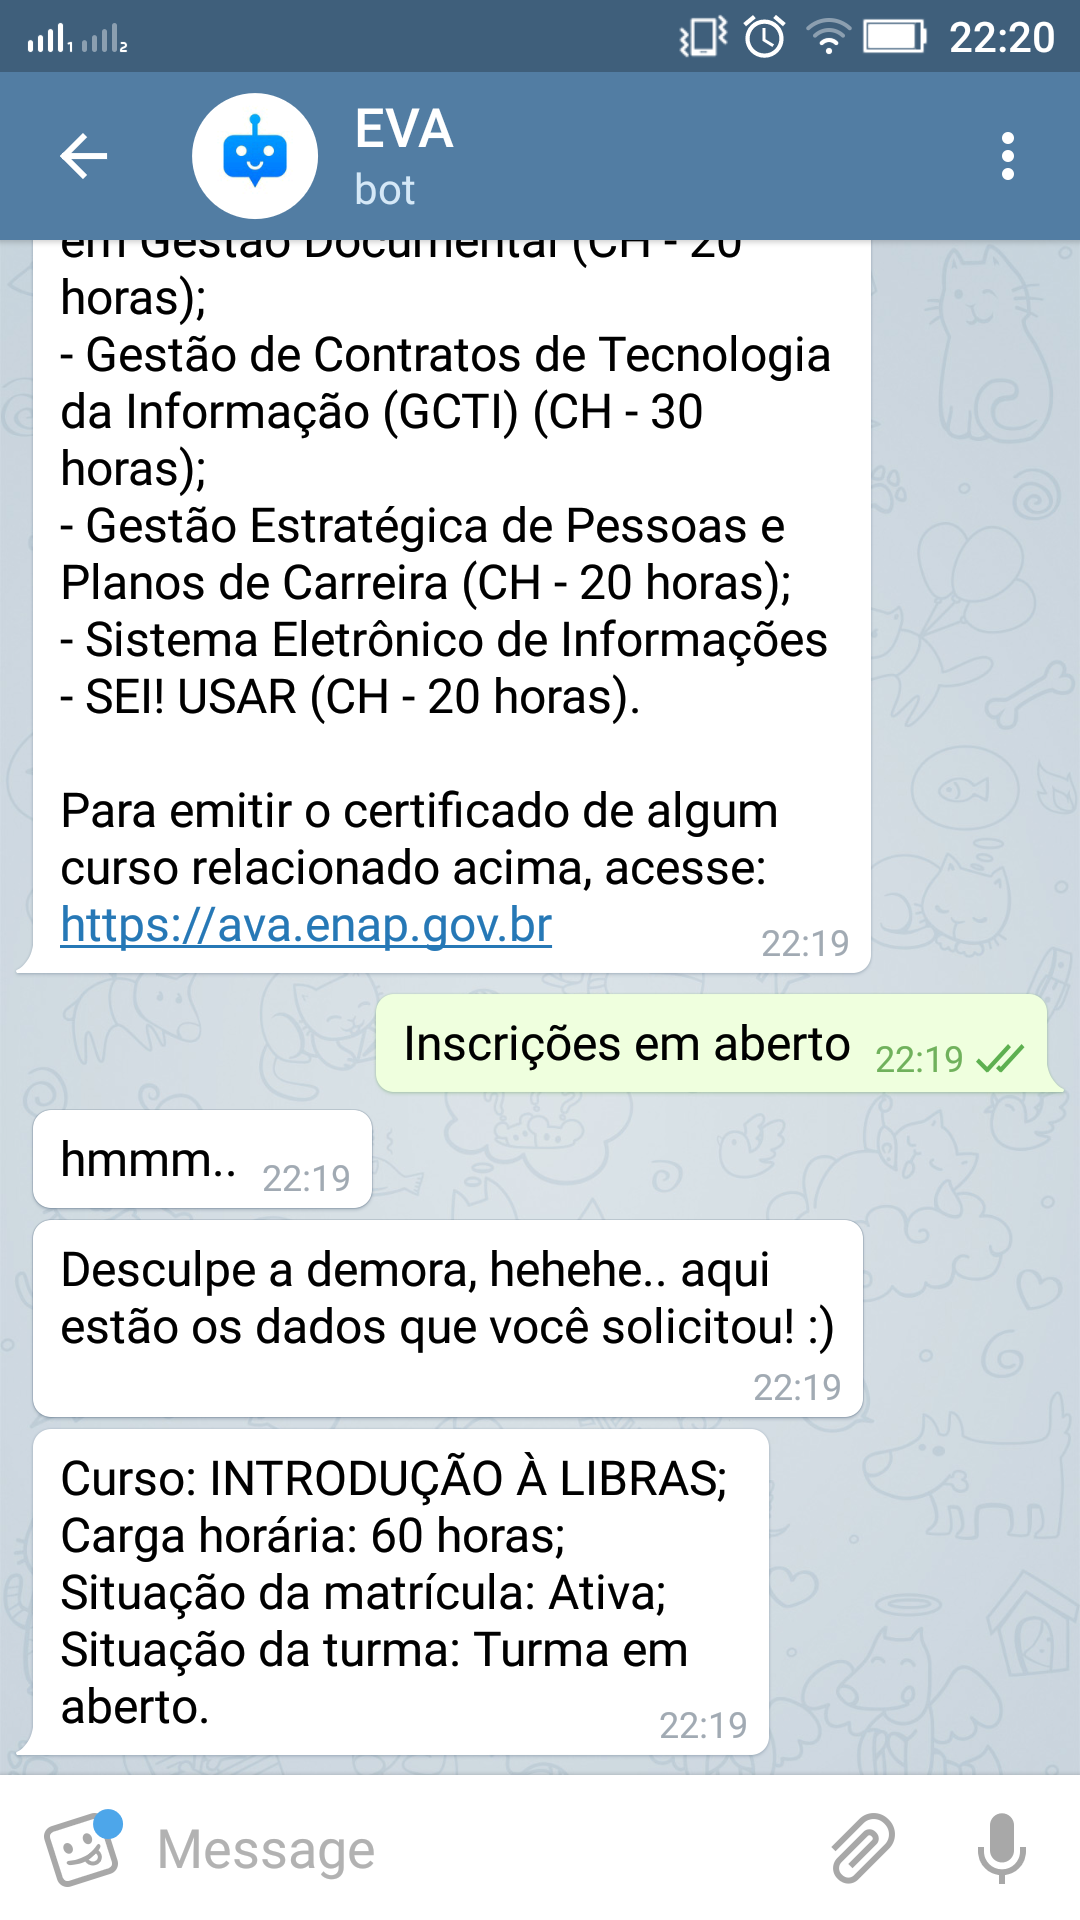
\includegraphics[width=0.2\linewidth]{src/imagens/apresentacao-cursos-aberto.png}
    \caption{EVA - Visualizando inscrições de cursos em aberto} Fonte: Elaborado pelo autor (2018)
    \label{cap:04:fig:apresentacao-inscricoes-aberto}
\end{figure}

\section{Desvinculando}

A qualquer momento, se for da vontade do aluno, ele poderá se desvincular do sistema de EVA, apenas enviando uma simples mensagem de texto, demonstrado na Figura \ref{cap:04:fig:apresentacao-logout}.

\begin{figure}[htb!]
    \centering
    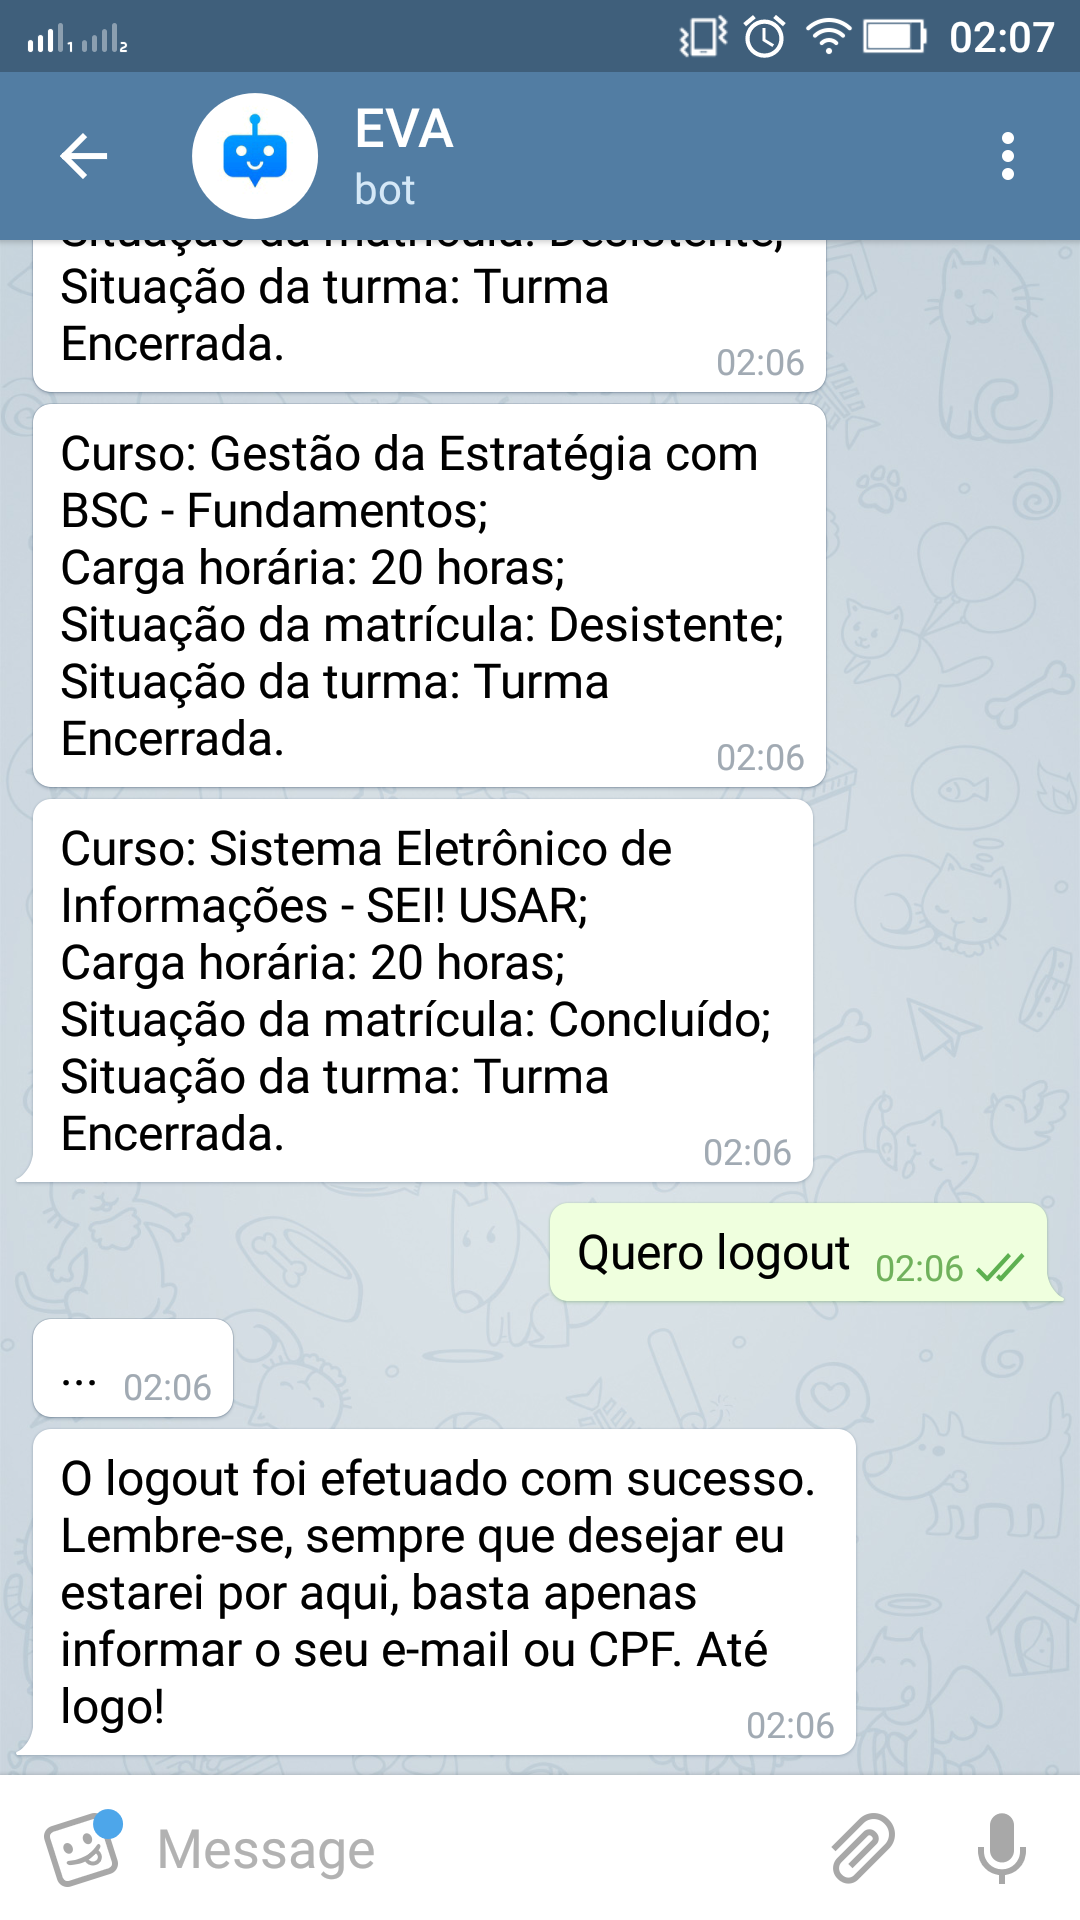
\includegraphics[width=0.2\linewidth]{src/imagens/apresentacao-logout.png}
    \caption{EVA - Logout} Fonte: Elaborado pelo autor (2018)
    \label{cap:04:fig:apresentacao-logout}
\end{figure}

  % Capitulo 5: Quinto capítulo (arquivo Includes/Capitulo5.tex)
  % Considera��es finais
\chapter{Considerações finais}

Oferecer um serviço massivo sem a devida capacidade de atendimento aos usuários representa um risco para a qualidade e a sustentabilidade do serviço prestado. De um lado, tem-se a insatisfação dos usuários causada pela falta de atendimento, e, de outro, a incapacidade do provedor de colher informações que são estratégicas para a melhoria contínua dos serviços e para a tomada de decisão.

No âmbito da EV.G, observa-se que grande parte das solicitações dos alunos referem-se a assuntos simples, repetitivos e facilmente resolvidos a partir de uma consulta a informações disponíveis em banco de dados. É o caso de dúvidas relativas à emissão de certificados, procedimentos de inscrição, credenciais de acesso, entre outros. Dúvidas qualitativas, referentes à conteúdos, situações inéditas, por exemplo, são raras e podem ser direcionadas para um atendimento de segundo nível.  

Com o avanço tecnológico, soluções inovadoras e de baixo custo estão surgindo a todo momento. No cenário do atendimento on-line, o uso de \textit{chatbots} é uma opção de baixo custo e alto desempenho. Como tal, o \textit{chatbot} é uma solução possível para atendimento massificado via algum método de conversação, como por exemplo em aplicações de mensagens instantâneas.

No contexto da EV.G, foi desenvolvido um \textit{chatbot} de conversação textual compatível com a plataforma mensagens instantâneas chamada Telegram, denominado EVA (EV.G Virtual Assistant). O objetivo geral de EVA é automatizar a interação via texto no atendimento administrativo de primeiro nível a alunos no âmbito da secretaria acadêmica da EV.G.

EVA é um \textit{chatbot} de domínio amplo, que possui a capacidade de interagir com os alunos vinculados ao EV.G na medida de suas necessidades. Em teoria, EVA não tem limite de atendimento simultâneo de alunos, nem tão pouco de horário de atendimento, por ser um programa de computador. O que torna ideal para atendimento em ambiente virtual de aprendizagem de alta disponibilidade, que é o caso da EV.G.

Por se tratar de um \textit{chatbot} de domínio amplo, EVA pode por meio de mecanismos de Inteligência Artificial, que para o seu caso utilizasse do PNL, aprender a partir das interações com os alunos e com isso, melhorar o seu repertório.

\section{Limitações}

O entendimento de EVA ainda é limitado devido ao seu pouco treinamento com base nas interações com os usuários do sistema, e também, devido as poucas intenções cadastradas e compreendidas durante a análise léxica, utilizando o PNL do Wit.ai. É válido ressaltar, que o Wit.ai oferece serviços para treinamento dos PNL desenvolvidos em sua plataforma, porém, devido ao escopo do presente trabalho, o treinamento realizado foi limitado às funcionalidades prioritárias requeridas pelo EV.G.

\section{Trabalhos futuros}

Espera-se que as funcionalidades de EVA possam continuar a serem desenvolvidas e melhoradas com o tempo, para que se possa atender as demandas dos alunos do EV.G, com ainda mais eficiência.

Um dos intuitos da criação da API de EVA, se deu justamente para facilitar que o sistema possa continuar crescendo, seja atendendo em outras plataformas de mensagens instantâneas, estabelecendo de uma interoperabilidade com outros serviços, e até mesmo para facilitar na implementação de novas funcionalidades de EVA. 

  \backmatter

  % Bibliografia (arquivo Capitulos/Referencias.bib)
  %\nocite{*}
  \postextual
  \bibliography{referencias}
  %\bibliographystyle{abnt-alf}

  % Apêndice A (arquivo Includes/ApendiceA)
%  \begin{apendicesenv}
    %\partapendices

%    % Ap�ndice
\apendice
\chapter{Primeiro apêndice}

Os apêndices são textos ou documentos elaborados pelo autor, a fim de
complementar sua argumentação, sem prejuízo da unidade nuclear do trabalho.

%  \end{apendicesenv}

  % Anexo A (arquivo Includes/AnexoA)
%   \begin{anexosenv}
%     \partanexos
%     % Anexo
\anexo
\chapter{Primeiro anexo}

Os anexos são textos ou documentos não elaborado pelo autor, que servem de
fundamentação, comprovação e ilustração.

%   \end{anexosenv}

\phantompart
\printindex

\end{document}
%--